\documentclass{article}

\usepackage[utf8]{inputenc}
\usepackage{enumerate} 
\usepackage{amsfonts}
\usepackage{amsmath}
\usepackage{amsthm}
\usepackage{blindtext}
\usepackage{graphicx}
\usepackage[numbers]{natbib}
\usepackage{amssymb}
\usepackage{mathtools}
\usepackage{stmaryrd}
\usepackage{tikz-cd}
 \usepackage{relsize}


\newtheorem{theorem}{Theorem}[section]
\newtheorem{lemma}{Lemma}[section]
\newtheorem{corollary}{Corollary}[section]
\newtheorem{conjecture}{Conjecture}[section]
\newtheorem{proposition}{Proposition}[section]
\theoremstyle{definition}
\newtheorem*{definition}{Definition}
\newtheorem{remark}{Remark}[section]
\newtheorem{experiment}{Experiment}[section]

\graphicspath{ {./images/} }
\numberwithin{figure}{section}



\title{An Introduction to the Toric Code as \\ Topological Quantum Computing}
\author{by Milo Moses}

\date{\textit{University of California, Santa Barbara} \\ [2ex] \today}


\begin{document}


\maketitle

\newcommand{\RR}{\mathbb{R}}
\newcommand{\HH}{\mathbb{H}}
\newcommand{\NN}{\mathbb{N}}
\newcommand{\QQ}{\mathbb{Q}}
\newcommand{\CC}{\mathbb{C}}
\newcommand{\FF}{\mathbb{F}}
\newcommand{\ZZ}{\mathbb{Z}}
\newcommand{\Ncal}{\mathcal{N}}
\newcommand{\TT}{\mathcal{T}}
\newcommand{\mm}{\mathfrak{m}}
\newcommand{\pp}{\mathfrak{p}}
\newcommand{\Hom}{\mathrm{Hom}}
\newcommand{\Frac}{\mathrm{Frac}}
\newcommand{\res}{\mathrm{res}}
\newcommand{\0}{\left|0\right>}
\newcommand{\1}{\left|1\right>}
\newcommand{\nullclass}{\left|\bold{0}\right>}
\newcommand{\alphaclass}{\left|\alpha\right>}
\newcommand{\betaclass}{\left|\beta\right>}
\newcommand{\alphabetaclass}{\left|\alpha\beta\right>}
\newcommand{\ppsi}{\left|\psi\right>}
\newcommand{\bigleadsto}{\mathlarger{\mathlarger{\mathlarger{\leadsto}}}}


\begin{abstract}
One of the most promising forms of quantum computation proposed today is Topological Quantum Computation. In this manuscript, we describe the simplest non-trivial example of Topological Quantum Computation: The toric code. We give explanations in terms of elementary mathematics and physics, as well as the high-power languages of Topological Quantum Field Theory and Modular Tensor Categories.
\end{abstract}

\newpage

\section{Preface}
\label{Preface}

In the last 30 years, prompted in large part by Peter Shor's discovery of an efficient factoring algorithm \cite{shor1994algorithms}, quantum computing has seen massive advances, and gained notoriety as an emerging technology and area of insight. However, nobody has yet been able to make a usable quantum computer. Precisely controlling this microscopic world has proved quite challenging. In particular, thermal fluctuations of the outside world cause quantum states to degenerate and scramble. For this reason, the current state of quantum computing research has been described as the ``NISQ era":  The noisy intermediate-scale quantum era.

To move past this requires some major insights and discoveries, and perhaps an entirely new model of quantum computation. One of the most recent such models is Topological Quantum Computation (TQC), proposed in a 2008 paper of Freedman-Kitaev-Larsen-Wang. The foremost team working on TQC is Microsoft Station Q, based in Santa Barbara, California. While this team has not been able to reliably perform computations with even a single qubit, they have made much progress since 2008. [WORK What was that progress?]

Surveys of TQC are few and far between. There are individually packaged references describing some of the relevant mathematics \cite{kauffman1994temperley, bakalov2001lectures, kauffman1994temperley}, some of the physics \cite{altland2010condensed, francesco2012conformal, wen2004quantum}, and some the abstract quantum-computation \cite{nielsen2002quantum, kitaev2002classical}. However, the only real holistic treatments are in Z. Wang's book \cite{wang2010topological}, and his article with E. Rowell \cite{rowell2018mathematics}. While certainly an important reference, one is expected to already have advanced knowledge of Algebraic Geometry, Category Theory, and Representation Theory. This text serves as a much more elementary entry point into this vast and intricate field. The most readable reference by far is \ref{freedman2002simulation}. [WORK: Restructure this paragraph. Ask Zhenghan.]

With a desire to remain as accessible as possible, we restrict ourselves to one of the simplest possible examples of TQC: The toric code. This special case is used as motivation for the general theory. Key concepts for the general picture are left undefined, for even simply stating the main results of general TQC would be too cumbersome, and lead us too far astray.

This manuscript is based on lecture notes from a course on TQC taught by Zhenghan Wang, in the winter of 2023 at UC Santa Barbara. The author expresses his sincerest gratitude to Zhenghan Wang and the other students of the class, without whom this manuscript would not have been possible.

The main reference for the first description of the toric code as a quantum system on the torus is the seminal work of Kitaev \cite{kitaev2003fault}. It was here that the idea of computation by braiding anyons was first described, and much of that paper focuses specifically on the example of the toric code as well.

Many of the propositions and descriptions offered are not anywhere to be found in literature. This is not due to them being particularly novel, but instead it is due to them being seen as too obvious to be stated explicitly, and are simply assumed as folklore. A secondary goal of this manuscript is to present a formal treatment of these implicit ideas.

Finally, we end with a terminological confusion. The term ``toric code" refers to an example of TQC, but also to an error correcting code in universal quantum computation. Moreover, it is from this use as an error correcting code that it gets the name ``toric code". A readable reference to the surface codes (a generalization of the toric code) as error correction can be found in J. Roffe's article \cite{roffe2019quantum}. The point is that TQC is so naturally error resistant, that its mathematical descriptions immediately give associated error correction algorithms. The widespread use and study of the toric code (the simplest non-trivial model!) outside of TQC can be seen as a testament to the power of the theory.


The structure of the manuscript is as follows:

\begin{itemize}
\item In Section \ref{Introduction}, we give an introduction to TQC. While great effort is taken to make the treatment as accessible as possible, one is still required to have at least an elementary understanding of mathematics and physics. A passing familiarity with quantum mechanics and quantum computation would be extremely useful.

\item in Section \ref{The Toric Code}, we give a mathematical description of the toric code in terms of undergraduate-level linear algebra. While not strictly necessary, having taken a first course in Algebraic Topology would be preferable. For those unfamiliar with the subject, an introduction is given in Appendix \ref{Homology}.

\item In Section \ref{TQFTs}...
\end{itemize}



\section{Introduction}
\label{Introduction}

Of the many approaches at quantum computation, Topological Quantum Computation (TQC) has the distinction of being both one of the most mathematically complicated and one of the most potentially powerful methods. In this manuscript, we describe the simplest non-trivial example of TQC: The toric code. While not being useful in itself (toric code TQC is far from being universal), a thorough understanding of the toric code undoubtedly elucidates the general TQC methodology.

To describe a theory of Quantum Computation, one describe the following:

\begin{enumerate}
\item How quantum information is stored (i.e, what physical model of qubits one is using)
\item How quantum information is acted on (i.e, what physical actions one can perform on the qubits)
\item How quantum information is measured (i.e, what observables can be physically measured in the system)
\end{enumerate}

A \textit{universal} model of quantum computation is one which can simulate all others. Generally, this will mean that the space of possible physical actions specified by the quantum computation model is dense in the space of all possible transformations on the space of qubits (i.e, can be used to approximate every transformation arbitrarily well).

While there are many proposed methods of quantum computation (superconducting quantum computers \cite{wendin2017quantum}, trapped ion quantum computers \cite{debnath2016demonstration}, semiconductor based quantum computers \cite{kane1998silicon}, etc...), it is expected that every such reasonable model will be essentially equivalent, in the sense that they can all \textit{effectively} simulate each other: This is the content of the Freedman-Church-Turing thesis \cite{freedman2003topological}.

In a a sequence of seminal works by Freedman, Kitaev, Larsen, and Wang, it was shown that universal quantum computers can effectively model any TQC, and conversely that there are models of TQC that can effectively simulate a universal quantum computer \cite{freedman2002modular} \cite{freedman2002simulation}.

If all forms of quantum computation are roughly equivalent it is reasonable to ask why one would consider TQC to be more promising than other models. This is an especially relevant question seeing as Google's superconducting quantum computer can harness 53 qubits and has demonstrated quantum superiority, but Microsoft's TQC has not been able to reliably harness a single qubit \cite{arute2019quantum}.

The intuition is as follows. The $\#$1 challenge in quantum computation is error correction. While fault tolerant quantum computers can probably exist (i.e, quantum computers that fix errors faster than they happen), the error rate must be un-physically low \cite{gottesman1998theory}. \textit{Topology} is the mathematical study of those properties of geometric objects that are invariant under small perturbations. The key insight of TQC is that instead of storing quantum information in the states of individual particles, the information is stored in topological invariants of geometric objects. As such, even when physical errors happen (i.e, the geometric object is perturbed) the information stored in the qubits remains the same. More than being error correcting, TQC is naturally error resistant!

As a thought experiment to reinforce this idea, suppose that Alice and Bob are placed across the country, and are given only a string to communicate. By ``string" we really mean string: This is some physical piece of twine or rope. They can ship this string via train, and through this process there will undoubtedly be errors (i.e, the string gets pushed around during the voyage). How can Alice and Bob effectively communicate, while being relatively confident there are no errors?

\begin{figure}
\begin{center}
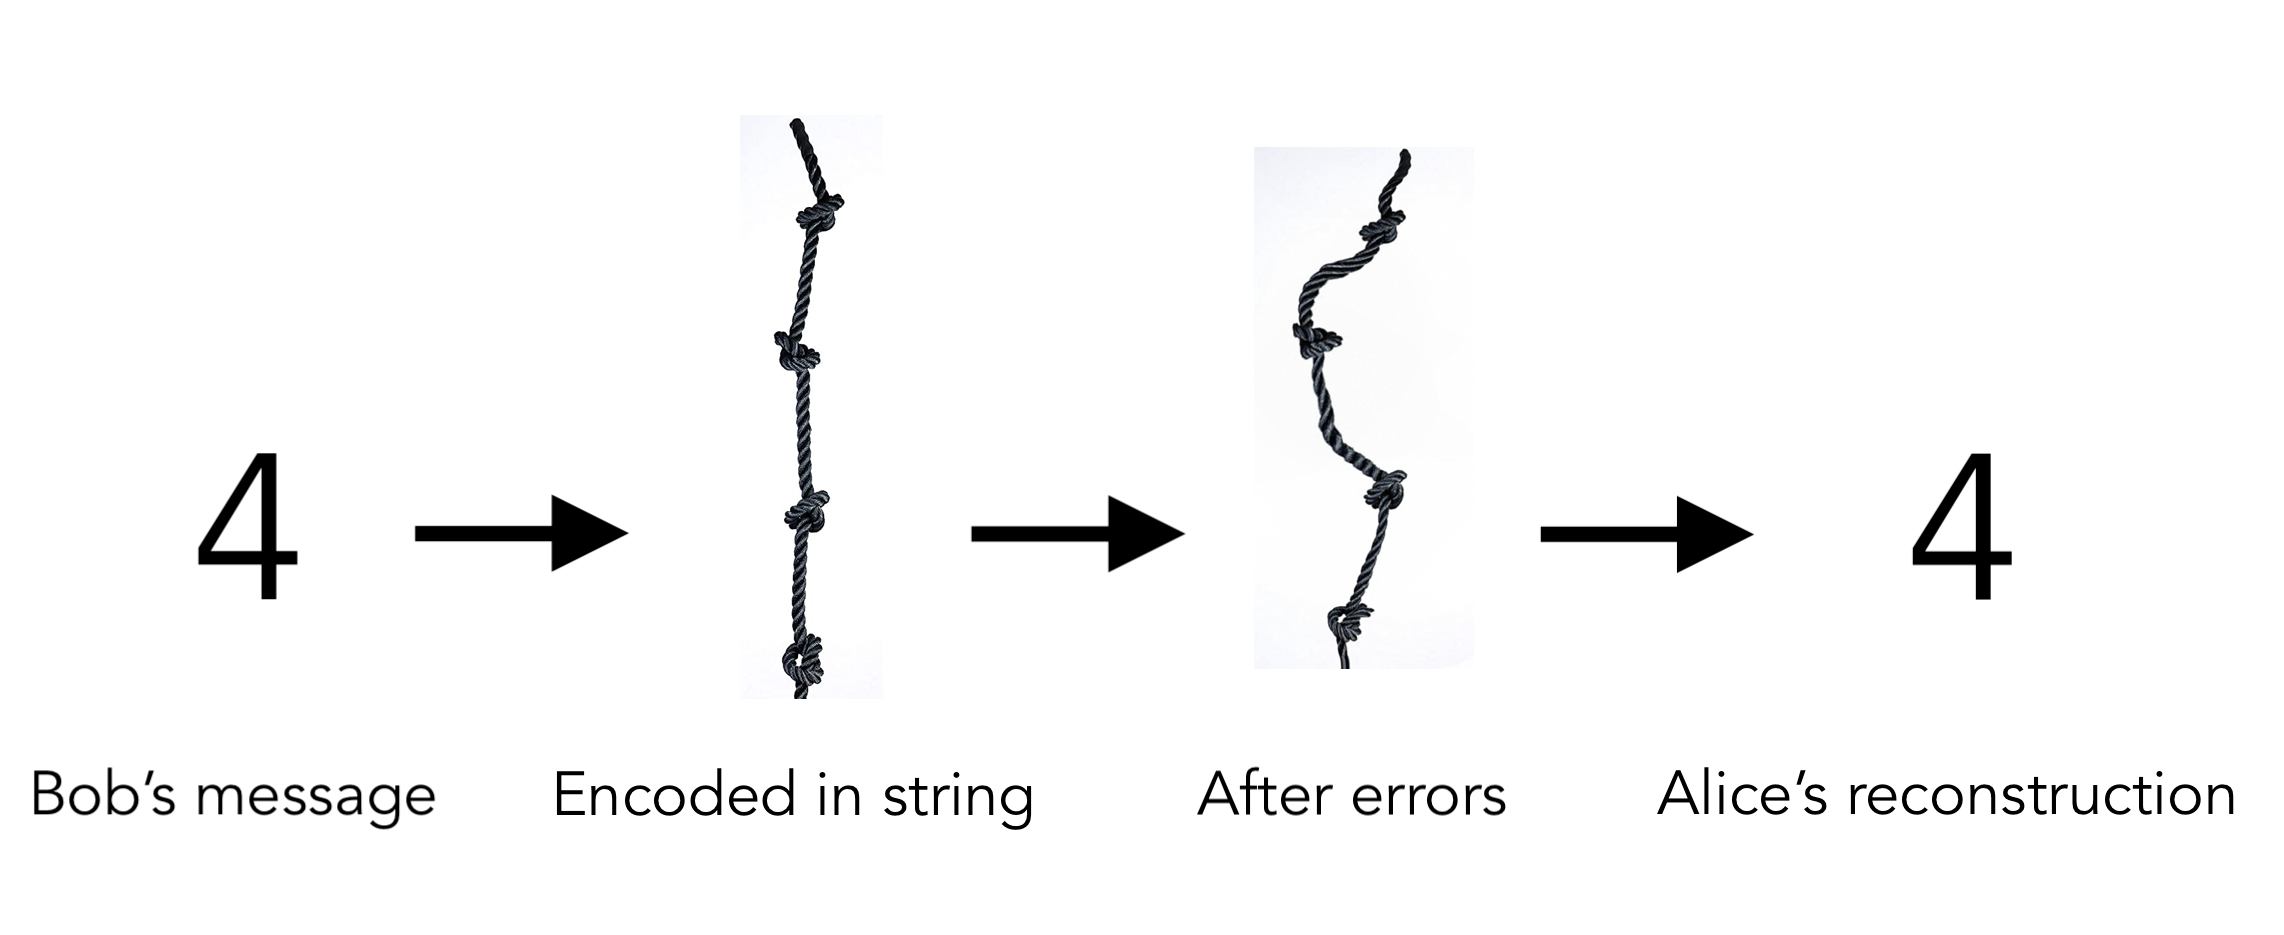
\includegraphics[scale=0.25]{rope-deformations}
\caption{A model of a (non-quantum) topological message}
\label{fig:rope-deformations}
\end{center}
\end{figure}

The answer is simple: Store the information in knots! By tying a certain number of simple knots in the string Alice can specify an integer, which Bob can simply read off by counting (as in Figure \ref{fig:rope-deformations})! The beauty is in the fact that while the string may have moved around during the sending process, it would take a very specialized and unlikely error to untie the rope or to accidently re-tie an extra knot. This knotting number is a topological invariant (small perturbations don't change how many knots were tied), and so we can see intuitively here that topological invariants are naturally error resistant.

Additionally, the above situation is more than just a thought experiment: This is exactly the scheme that the ancient South American Incas used over 4000 years ago! The Incas stored all sorts of information in \textit{Quipus}, intricately knotted collections of fibered strings \cite{ascher1981code}, as seen in Figure \ref{fig:quipu}. Storing information in knot invariants was also common practice in ancient Chinese, Tibetan, and Polynesian cultures \cite{day2021quipus}. In some sense, these are the earliest examples of topological computation.

\begin{figure}
\begin{center}
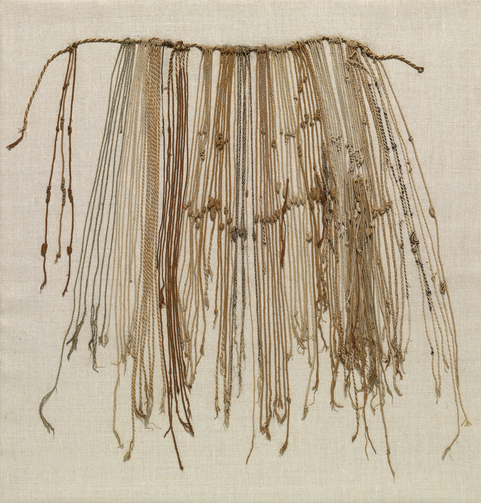
\includegraphics[scale=0.85]{quipu}
\caption{An Incan Quipu}
\label{fig:quipu}
\end{center}
\end{figure}


In TQC, information is still stored in knots. The main difference is that the strings being knotted are no longer physical pieces of twine, but \textit{trajectories of quasiparticles through spacetime}. For instance, suppose $X$ and $Z$ are two quasiparticles (we will elaborate more on this in later). Moving through space from time $t_0$ to $t_1$, the trajectories can look something like Figure \ref{fig:braiding}. Quantum interactions cause the knotting to yield real differences in physical states, and hence these knots can be used to store quantum information.

\begin{figure}
\begin{center}
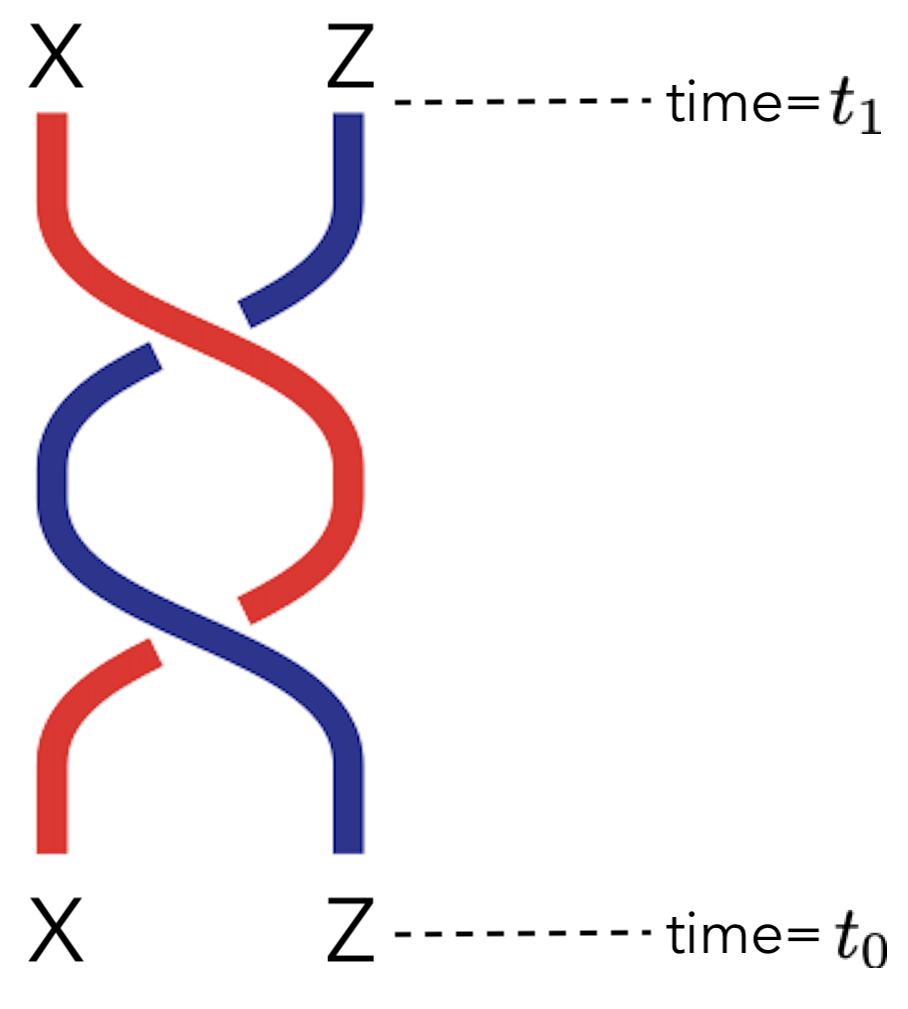
\includegraphics[scale=0.25]{braiding}
\caption{Braiding of quasiparticles in spacetime}
\label{fig:braiding}
\end{center}
\end{figure}


Notice that to make a 3 dimensional spacetime, we are modeling space as being 2 dimensional. While one might initially think this is a quirk of our human incapacity of visualizing 4 dimensional space, there is a deeper mathematical truth here: There are no knots in 4 dimensional space. The extra dimension always gives the strands space to evade and move past each other without collision. In particular, for TQC to work we must have space be two dimensional. While this task seems initially impossible, (essentially) two dimensional quantum phases of matter have been experimentally constructed. Things that behave like particles in these 2 dimensional phases of matter are known as quasiparticles, and form non-trivial knots when braided.

A rough description of how these 2 dimensional electron gasses are constructed is described as follows. One begins by preparing a series of layers of graphene with a small gap in the middle. Upon subjecting the system to extremely cold temperatures and an extremely high magnetic field, the electrons in the graphene begin to move around. To balance the electric charge on both sides, all of the electrons move to the exact center of the setup. This resulting thin layer of electrons is the two dimensional electron gas. In such extreme conditions, all of the electrons will become highly entangled with each other, forming a quantum phase of matter \cite{yang2021experimental}.

A key insight of Kitaev \cite{kitaev2003fault}, and one of the motivating pushes towards quantum computation, was that the topological properties of the 2 dimensional phase of matter will determine how the electrons entangled with each other. In other words, 2 dimensional sheets of electrons will quantize differently depending on their shape.

To understand this better, suppose that you have a 2 dimensional sphere of electrons. They will want to quantize, and align their spins together in the same direction. This amounts to choosing a unit tangent vector at each point on the sphere. However, there is no coherent way to do this. Every choice of tangent vectors will necessarily have some discontinuity or singularity: This is the content of the ``Hairy Ball Theorem".

If your sheet of electrons was on a donut, however, the situation is much different. There are several ways of assigning unit tangent vectors coherently to each point, and thus there are several ways for all of the electrons to quantize their spins together, as seen in Figure \ref{fig:hairy-ball}. This is aptly known as a \textit{spin liquid}. In mathematical language, a ``donut" is called a torus, hence the name \textit{toric code}. The spin liquid associated with this procedure on a torus is called the ``$\ZZ_2$ spin liquid", and it is the physical realization of the toric code. We will spend the body of this manuscript describing the mathematics of the toric code in more detail. Note that generally when making such $\ZZ_2$ spin liquids in labs one does not make an actual torus; instead, one artificially simulates the boundary conditions of a torus, for technical reasons.

\begin{figure}
\begin{center}
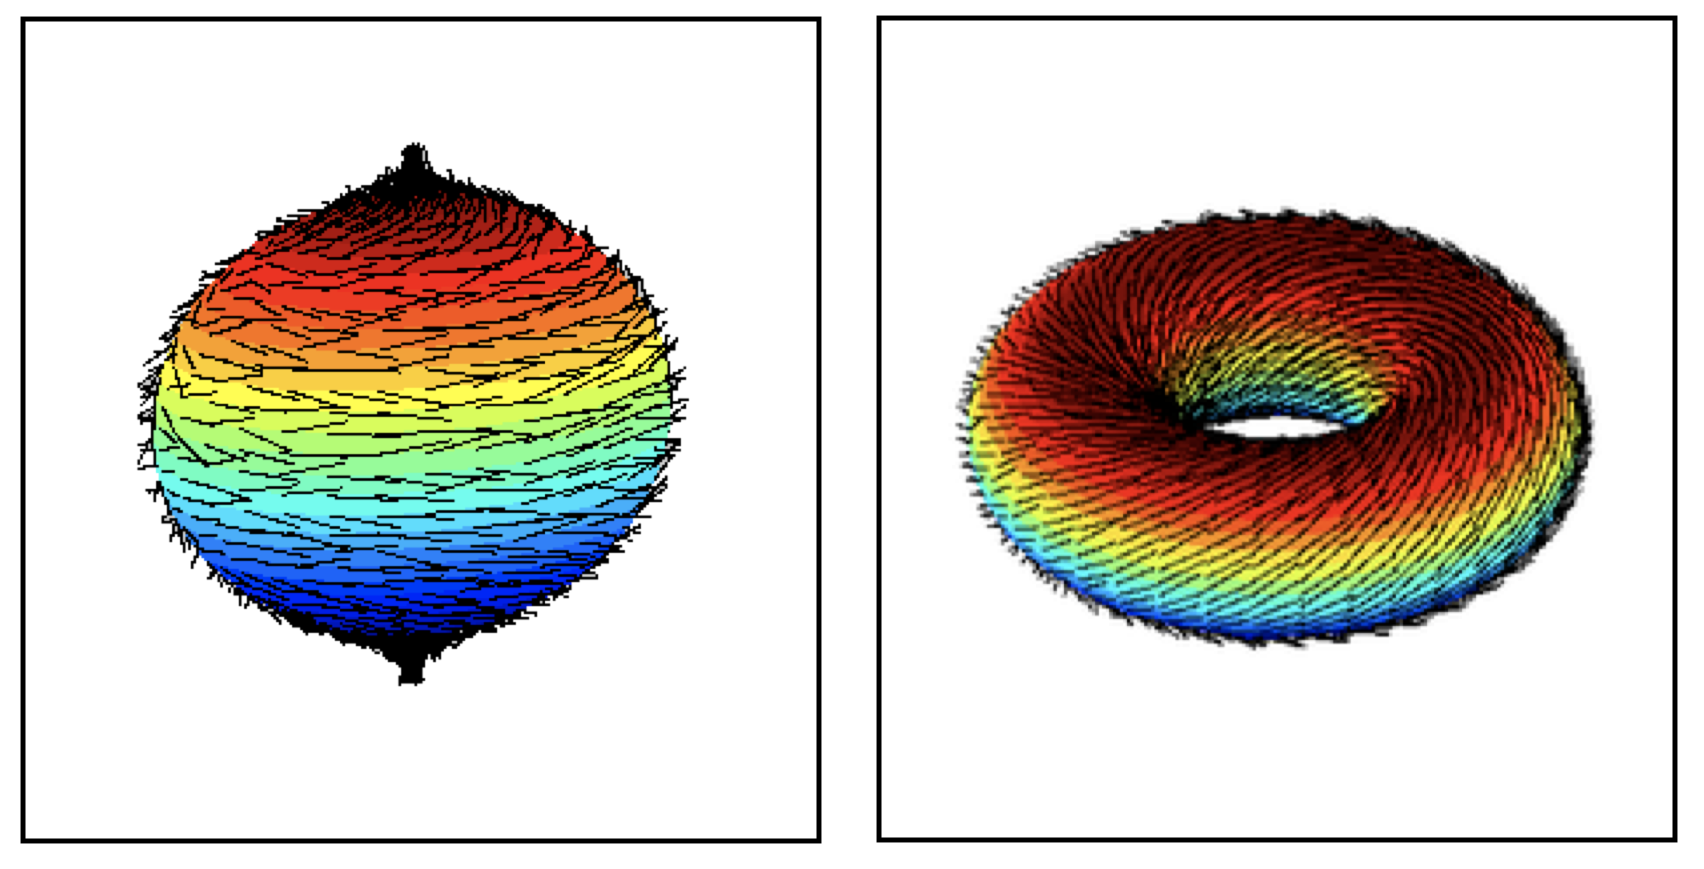
\includegraphics[scale=0.2]{Hairy-Ball-Diagram}
\caption{Assigning vector fields (spins) to a sphere, verses to a torus}
\label{fig:hairy-ball}
\end{center}
\end{figure}


We find it illustrative here to make an analogy with classical computing. Namely, there is the following puzzle: Classical bits are stored in the magnetization of small regions on a hard disk. The magnetization of each atom is highly sensitive to thermal fluctuations, and so one might ask why it is that classical computers seem so resistant to errors. The answer is that since all of the atoms are magnetized in the same direction, any one atom flipping will automatically be corrected back by the normalizing influence of the other atoms: magnets are naturally error resistant. It is exactly the same with these spin liquids that quantize together: Any one electron's spin decohering will immediately be corrected by the normalizing influence of all of its neighbors.

Before moving on to an in-depth treatment of the toric code, we offer a general description of the TQC process, in the style of the three points listed in the beginning of the introduction:

\begin{enumerate}
\item Information is stored in the ground states of topological quantum materials.
\item Ground states are acted on by braiding of quasiparticles, that is, by generating pairs of quasiparticles and making them knot in spacetime.
\item Measurement is performed by observing the topological properties of the resulting ground state.
\end{enumerate}

Here, \textit{ground state} refers to a state in the system with lowest possible energy. Note that in the previous description of spin liquids, all electrons having the same spin is a result of them being in the lowest energy state. An ``excited" electron with deviant spin will raise the energy of the system. In this way, quasiparticles can be interpreted as excitations of the topological quantum material. Note additionally this motivates the fact that (topological) quantum computers must be exceptionally cold to function: Any extra energy will correspond to extra excitations, causing the computer to malfunction, since by definition the states information is stored in are ground states.

The possibilities for topological quantum materials and TQC are extremely exciting, and we are eager to see where the field will go in the coming years.

\section{The Toric Code}
\label{The Toric Code}

Consider a torus. We will be imagining the torus as a whole as being a quantum system, corresponding physically to the quantum system one would observe when the torus is in the $\ZZ_2$ spin liquid topological quantum phase of matter. The \textit{code space} of the torus is the space of states on which we will be building our quantum computer, i.e, those states we will be using to store quantum information. In general Topological Quantum Computing (TQC) fashion, the code space of the toric code will be its ground states.

Our mathematical priorities are thus as follows: To define the quantum system, and to define a Hamiltonian operator on it. A Hamiltonian is an operator corresponding to the total energy of a quantum system. Namely, the eigenvalue of an eigenstate of the Hamiltonian corresponds to the total energy of that state. The code space will thus be the lowest eigenspace of the Hamiltonian.

\begin{figure}
\begin{center}
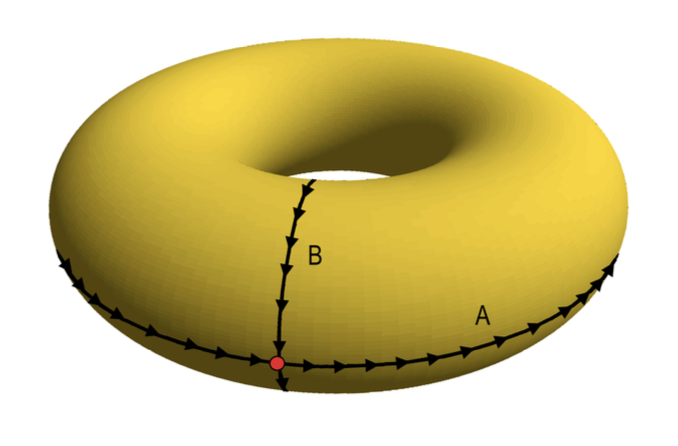
\includegraphics[scale=0.3]{torus}
\caption{Celluation of the torus, obtained by gluing opposite sides together.}
\label{fig:torus}
\end{center}
\end{figure}

Working with a continuous torus and the corresponding infinite dimensional vector spaces is cumbersome and unnecessary. Instead, we celluate the torus into an $n$ by $n$ square lattice with opposing sides identified, as in Figure \ref{fig:torus}. We will work with the understanding that the real physical system is the limit as $n\to\infty$. We define the quantum system associated with the $n$ by $n$ celluated torus to be the vector space

$$\Ncal=\bigotimes_{\substack{\text{edges of}\\\text{torus}}}\CC^2,$$

obtained by ``putting a qubit
\footnote{A qubit is the quantum-computing term for ``two dimensional quantum system", i.e, $\CC^2$.}
on every edge". Here and throughout, \textit{vertices}, \textit{edges}, and \textit{faces}, when used as indexing sets, will refer to the set of \textit{vertices}, \textit{edges}, and \textit{faces} of our celluated torus. We will choose a canonical basis $\left\{\0,\1\right\}$ for $\CC^2$, reflecting our information theoretic intentions. To more forward with defining the Hamiltonian, we introduce the Pauli matrices

$$
\sigma_X=
\begin{pmatrix}
0 & 1\\
1 & 0
\end{pmatrix},\,\,
\sigma_Y=
\begin{pmatrix}
0 & -i\\
i & 0
\end{pmatrix},\,\,
\sigma_Z=
\begin{pmatrix}
-1 & 0\\
0 & 1
\end{pmatrix}.
$$

The Hamiltonian is defined by

$$H=-\sum_{\text{vertices } v}A_v-\sum_{\text{faces } p}B_p,$$

where

$$A_v=\bigotimes_{\substack{\text{edges}\\ \text{touching }v}}\sigma_Z,\,\, B_p=\bigotimes_{\substack{\text{edges}\\ \text{touching }p}}\sigma_X.$$

All of the power of the toric code comes from this highly non-obvious choice of Hamiltonian. The physical interpretation for this choice of Hamiltonian comes from gauge theory. Namely, the $U(1)$ Lattice Gauge Theory has two fields: The Compact Gauge Field and the Electric Field. Exponentiating the Compact Gauge Field we get the $\sigma_X$ operators, and exponentiating the Electric Field we get the $\sigma_Z$ operators. Thus, the $A_v$ contribute a ``Gauss' Law" term, and the $B_p$ contribute a ``Magnetic Field" term to the Hamiltonian \cite{oh2022rank}. While potentially physically illuminating, this discussion of gauge theory will have no influence on the rest of the mathematics presented in this manuscript, and does not need to be understood to appreciate the toric code.

Letting $I$ denote the identity matrix, the key facts about the $A_v$s and $B_p$s are summarized in the following proposition:

\begin{proposition}\label{AvBp}We have that

\begin{enumerate}[(i)]
\item $A_v^2=B_p^2=I$ for all $v,p$
\item All $A_v$s and $B_p$s have half eigenvalues $+1$ and half eigenvalues $-1$
\item All $A_v$s and $B_p$s commute
\item $\prod_{\text{vertices }v}A_v=I$ and $\prod_{\text{faces }p}B_p=I$
\end{enumerate}

\end{proposition}
\begin{proof}
$(i).$ Multiplying tensor product matrices corresponds to simply multiplying componentwise. Hence, this part  follows immediately from the relations $\sigma_X^2=\sigma_Z^2=I$.

$(ii).$ We define an isomorphism between the $+1$ eigenspace and $-1$ eigenspace of $A_v$. Namely, apply $\sigma_X$ to  an edge $e$ touching $v$. Since $\sigma_X\sigma_Z=-\sigma_Z\sigma_X$, the computation

$$A_v \left(\bigotimes_{\text{edge }e}\sigma_X\right)\ppsi = -A_v \left(\bigotimes_{\text{edge }e}\sigma_X\right)A_v\ppsi $$

show that a $+1$ eigenstate will be transformed into a $-1$ eigenstate, and a $-1$ eigenstate will be turned into $+1$ eigenstate. Thus, this defines an isomorphism between the desired eigenspaces. Applying $\sigma_Z$ instead of $\sigma_X$, we can define a similar isomorphism for $B_p$.

this will have the effect of turning a $+1$ eigenstate into a $-1$ eigenstate and vice-versa,

$(iii).$ All the $A_v$s commute with each other since $\sigma_Z$ commutes with itself, and all the $B_p$s commute with each other since $\sigma_X$ commutes with itself. What's left to check is that $A_vB_p=B_pA_v$. Notice that if $v$ is not touching the face $p$, none of the $\sigma_Z$s in the tensor product of $A_v$ will be in the same spots as any of the $\sigma_X$s as the tensor product for $B_p$. Hence, $A_v$ and $B_p$ commute in this case. If $v$ is touching $p$, then exactly two of the $\sigma_Z$s in the tensor product of $A_v$ will be in the same spots as $\sigma_X$s in the tensor product of $B_p$. Hence, pulling $B_v$ through $A_v$ corresponds to switching $\sigma_X$ and $\sigma_Z$. Since $\sigma_X\sigma_Z=-\sigma_Z\sigma_X$, this introduces an overall phase shift of $(-1)^2=1$. Hence, $A_vB_p=B_pA_v$ as desired!

$(iv).$ Applying $\prod_{\text{vertices } v}A_v$, is the same as applying $\sigma_Z$ to each vertex $2$ times, since each edge touches exactly $2$ vertices. Hence,

$$\prod_{\text{vertices } v}A_v=\bigotimes_{\text{edges}}\sigma^2_Z=\bigotimes_{\text{edges}}I=I.$$

Similarly, since every edge touches exactly $2$ faces, the fact that $\prod_{\text{faces } p}B_p=I$ follows from $\sigma^2_X=1$.
\end{proof}

Using the above facts about the $A_v$s and $B_p$s, we can describe the eigenspaces of $H$ well enough to compute their dimension:

\begin{proposition}\label{eigenspaces} All eigenvalues of $H$ are of the form $-2n^2+4q$, for an integer $q\leq n^2/2$. The $-2n^2+4q$ can be described as the space of states $\ppsi$ such that

$$\left|\left\{\left. v,p\right| A_v\ppsi =-1,\,\, B_p\ppsi=-1\right\}\right|=2q,$$

that is, the space of states with $2q$ excitations. There will always be an even number of $v$ such that $A_v\ppsi =-1$, as well as an even number of $p$ such that $B_p\ppsi=-1$. The dimension of of this eigenspace is

$$4\sum_{k=0}^{q}{n^2 \choose 2k} {n^2 \choose 2(q-k)}.$$

In particular, the code space of the toric code is 4 dimensional, and consists of those vectors $\ppsi$ such that $A_v\ppsi=B_p\ppsi=\ppsi$ for all $v,p$.
\end{proposition}
\begin{proof} To begin, we observe the following general fact from linear algebra. If $M$ and $N$ are commuting matrices and $\ppsi$ is an eigenvector for $N$ with eigenvalue $\lambda$, then

$$N(M\ppsi)=M(N\ppsi)=\lambda (M\ppsi).$$

Hence, $M$ respect the eigenspaces of $N$, and vice versa. This implies that the eigenspaces for $H$ will be simultaneous eigenspaces for all of the $A_v$s and $B_p$s, since all of the $A_v$s and $B_p$s commute by Proposition \ref{AvBp} (iii).

Suppose that $\ppsi$ is an eigenstate with

$$\left|\left\{\left. v,p\right| A_v\ppsi =-1,\,\, B_p\ppsi=-1\right\}\right|=q.$$

Then, we find that

\begin{align*}
H\ppsi&=(-\sum_{v}A_v-\sum_{p}B_p)\ppsi\\
&=\left(\sum_{\substack{v,p \\ -1\text{ eigenvalue}}}1-\sum_{\substack{v,p \\ 1\text{ eigenvalue}}}1\right)\ppsi\\
&=(q-(n^2-q))\\
&=-n^2+2q.
\end{align*}

Thus, to complete the initial description of the eigenstates, we must show that the number of $v$ such that $A_v\ppsi=-1$ and the number of $p$ such that $B_p\ppsi=-1$ is even. This follows from the computation that is this number where odd, then we would have by Proposition \ref{AvBp} (iv) that

$$\ppsi = \left(\prod_{v}A_v\right) \ppsi = -\ppsi,$$

which is a contradiction since we are supposing that $\ppsi\neq 0$. The exact same argument applies to the $B_p$. We now compute the dimensions of the eigenspaces. Let $D$ denote the dimension of the group space. We show that given any even sized sets $\bold{v}, \bold{p}$ of vertices and faces respectively, the space

$$\Ncal_{\bold{v},\bold{p}}=\{\left.\ppsi\right| \left(A_v\ppsi=-1\iff v\in \bold{v}\right),\,\, \left(B_p\ppsi=-1\iff p\in\bold{p}\right) \}$$

is $D$ dimensional. We proceed by induction on $|\bold{v}+\bold{p}|$. If $|\bold{v}+\bold{p}|=0$, then this is the definition of $D$. Without loss of generality, suppose $|\bold{v}|\geq 2$. If $|\bold{p}|\geq 2$, we apply the same arguement with verticies replaced by faces. Choose two verticies $v_0,v_1\in \bold{v}$. Choose a path $\gamma$ along the edges of the torus that connect $v_0$ and $v_1$. We show that $\bigotimes_{\text{edges in }\gamma}\sigma_X$ gives an isomorphism between $\Ncal_{\bold{v},\bold{p}}$ and $\Ncal_{\bold{v}-\{v_0,v_1\},\{p\}}$. Namely it is clear from $\sigma_X^2=\sigma_X$, so this map is its own inverse, so it is sufficient to show that the image is in the desired space. To prove this, we observe that $\bigotimes_{\text{edges in }\gamma}\sigma_X$ commutes with all the $B_p$s, and commutes with all of the $A_v$s at verticies that $\gamma$ passes through an even number of times. The only verticies that $\gamma$ passes through an odd number of times are its endpoints (by definition), and hence $A_v$ has exactly the effect of flipping the eigenvalues at $A_{v_0}$ and $A_{v_1}$. Thus, the image of a point in $\Ncal_{\bold{v},\bold{p}}$ is in $\Ncal_{\bold{v}-\{v_0,v_1\},\bold{p}}$, as desired.

Combining, we find that the $-2n^2+2q'$ eigenstate can be decomposed as direct sums of $\Ncal_{\bold{v},\bold{p}}$, where $\bold{v}$ and $\bold{p}$ range over even sized sets with $|\bold{v}+\bold{p}|=q'$. In particular, $q'=2q$ must be even. The dimension of this space is equal to $D$ times the number of way of choosing the sets $\bold{v}$ and $\bold{q}$, i.e,

$$D\sum_{k=0}^{q}{n^2 \choose 2k}{n^2 \choose 2(q-k)}.$$

The total dimension of eigenspaces of $H$ can be computed as

\begin{align*}
D\sum_{q=0}^{2n^2}\sum_{k=0}^{q}{n^2 \choose 2k}{n^2 \choose 2(q-k)}&=D\left(\sum_{q=0}^{2n^2}{n^2 \choose 2k_0}\right)\\
&=D\cdot \left(2^{n^2-1}\right)^2=D\cdot 2^{2n^2-2}.
\end{align*}

The Hamiltonian is a symmetric matrix with real coefficients, since it is the tensor product of such matrices. It is a standard fact from linear algebra that such matrices can be diagonalized, and hence the total dimension $H$ is equal to the dimension of $\Ncal=\bigotimes_{\text{edges}}\CC^2$. Seeing as there are $2n^2$ edges this space is $2^{2n^2}$ dimensional, and hence we must have $D=2^2=4$.
\end{proof}

The fact that the code space is four dimensional can be motivated as follows. By Proposition \label{AvBp} (ii), being in the $+1$ eigenspace for each $A_v$ and $B_p$ will impose a condition that decreases the dimension of your space by $1/2$. Since $\Ncal$ is $2^{2n^2}$ dimensional, imposing all $n^2$ of these conditions decreases the code space to $1$ dimension. However, the fact that $\prod_{\text{vertices }v}A_v=I$ and $\prod_{\text{faces }p}B_p=1$  from Proposition \label{AvBp} (iv) shows that two of these conditions imposed were redundant, brining the code space dimension back up to $2^2=4$ dimensions.

To describe the generators of the codespace explicitly we will need to use the basics of homology theory with $\ZZ_2$ coefficients, where $\ZZ_2=\{0,1\}$ is the additive group modulo $2$. For those unfamiliar, a brief introduction is included in Appendix \ref{Homology}.

\begin{figure}
\begin{center}
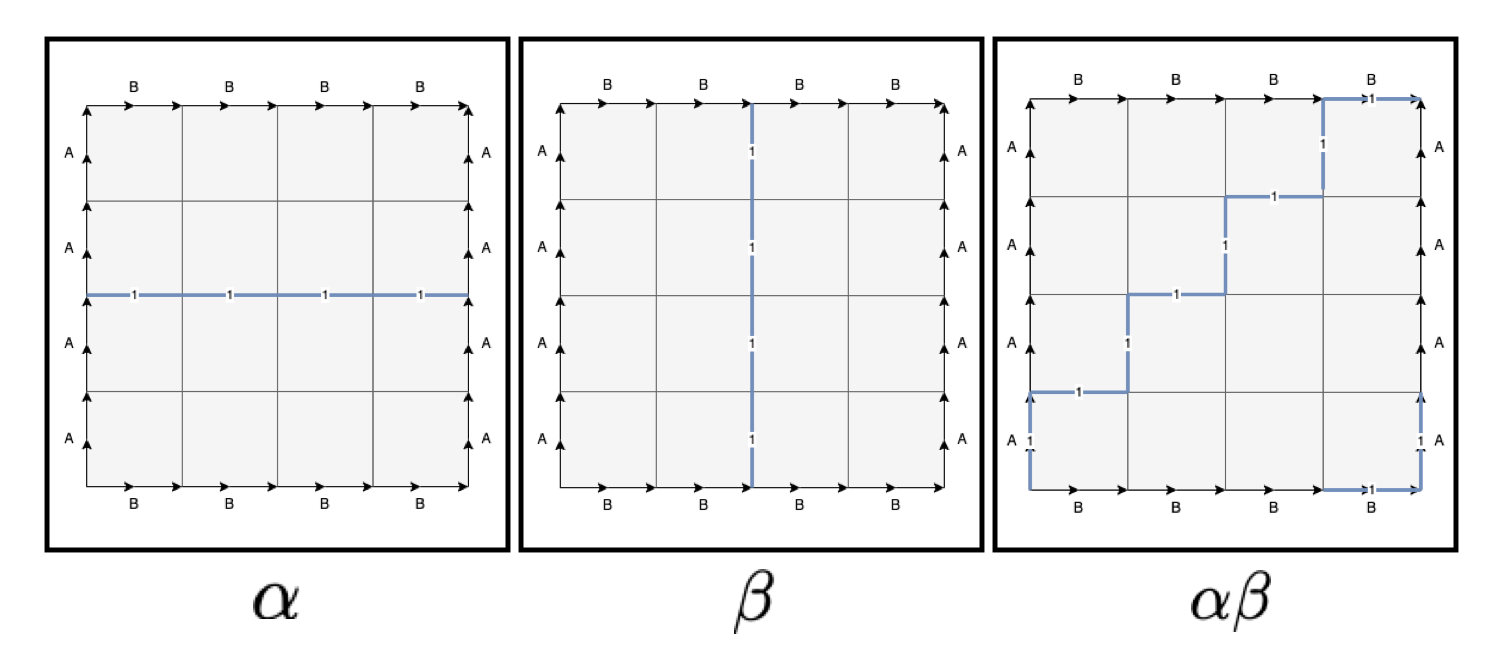
\includegraphics[scale=0.4]{homology-classes}
\caption{The three non-trivial homology classes of a torus}
\label{fig:homology}
\end{center}
\end{figure}


A pure state on $\Ncal$ is specified by a pure state on each qubit, namely, a choice of $\0$ and $\1$ for each edge. This is exactly the data to specify a $\ZZ_2$-chain. Given a $\ZZ_2$-chain $\gamma$, we write $\left|\gamma\right>$ for the associated pure state. Given any $\gamma,\gamma'$, we write $\gamma\sim \gamma'$ to mean that $\gamma$ and $\gamma'$ are homologous. The following elucidates the meaning of the codespace of the toric code:

\begin{proposition}\label{basis} Let $\bold{0},\alpha,\beta,$ and $\alpha\beta$ be the four $\ZZ_2$ homology classes on the torus, as in Figure \ref{fig:homology}. Choose $\bold{0}_0$, $\alpha_0$, $\beta_0$, and $(\alpha\beta)_0$ respectively to be representatives. Then, letting $\gamma$ run over all $\ZZ_2$-cycles, we have that

\begin{align*}
\nullclass &= \frac{1}{\sqrt{2^{n^2-1}}}\sum_{\gamma\sim \bold{0}_0}\left|\gamma\right>,\,\, \alphaclass=\frac{1}{\sqrt{2^{n^2-1}}}\sum_{\gamma\sim \alpha_0}\left|\gamma\right>,\\
\betaclass &= \frac{1}{\sqrt{2^{n^2-1}}}\sum_{\gamma\sim \beta_0}\left|\gamma\right>,\,\, \alphabetaclass=\frac{1}{\sqrt{2^{n^2-1}}}\sum_{\gamma\sim (\alpha\beta)_0}\left|\gamma\right>,
\end{align*}

are all normalized eigenstates of that Hamiltonian $H$, and serve as a canonical orthonormal basis of the codespace.
\end{proposition}
\begin{proof} Choose $\omega\in H_1(T;\ZZ_2)$. To show that $\left|\omega\right>$ is in the codespace, we observe that it is in the $+1$ eigenspace of every $A_v$ and $B_p$. Since $\sigma_Z$ sends $\0$ to $\0$ and $\1$ to $-\1$, $A_v$ has the effect of sending a pure state $\left|\gamma\right>$ to $\pm\left|\gamma\right>$, depending on whether $\gamma$ has an odd or even count of edges touching the vertex $v$. In particular, because $\gamma$ is running over cycles, we have that each $\left|\gamma\right>$ is in the $+1$ eigenspace of all the $A_v$, and hence the same applies to $\left|\omega\right>$.

For $B_p$s, we observe that applying $B_p$ to a pure state $\left|\gamma\right>$ has the effect of flipping all of the qubits around the face $p$. By definition of being $\ZZ_2$ homologous, $B_p$ maps the space of all cycles homologous to $\left|\omega\right>$ back into the space of all cycles homologous to $\left|\omega\right>$. In particular, $\left|\omega\right>$ is in the $+1$ eigenspace of $B_p$ for every $p$.

To show that $\left|\omega\right>$ is normalized, we observe that there are exactly that there are exactly $2^{n^2-1}$ cycles homologous to $\omega$. This is proved as follows. Starting with a fixed representative $\omega_0$ of $\omega$, cycles homologous to $\omega$ correspond to flipping qubits around the edges, i.e, applying $B_p$s at faces. Since there are $n^2$ faces, this gives $2^{n^2}$ cycles. This overcounts the space of cycles homologous to $\omega$ by a factor of $2$, since $\prod_{\text{faces }p}B_p=I$ by Proposition \ref{AvBp} (iv). The fact that the codespace is 4 dimensional says that this is the \textit{only} relation between the $B_p$s. Hence, there are $2^{n^2-1}$ cycles.

To show that these states are mutually orthogonal, we observe simply that no cycle can be homologous to two of the $\{\bold{0},\alpha,\beta,\alpha\beta\}$, hence $\left\{\nullclass,\alphaclass,\betaclass,\alphabetaclass\right\}$ have disjoint support, hence they are orthogonal.
\end{proof}

Letting $T$ denote the torus, the above shows that we can view the codespace of the toric code as a physical realization of the vector space $\CC[H_1(T;\ZZ_2)]=H_1(T,\CC)$. Here, $\CC[A]$ for some set $A$ denotes the vector space generated by $A$, i.e, the unique complex vector space which has a basis given by $A$. Quantum physics gives the physical analogue of the abstract mathematical notation of an equivalence class, namely, an equivalence class is realized as the superposition over all possible representatives. This can be compared with the path integral formulation of quantum mechanics, where one integrates over all possible paths between two points.

We now give \textit{quasiparticle} interpretation of the toric code. A quasiparticle is an excitation in the toric code. Namely, given an eigenstate $\ppsi$, we say that there is a quasiparticle at a vertex $v$ if $A_v\ppsi=-\ppsi$, and get a face $p$ we say that there is a quasiparticle at $p$ if $B_p\ppsi=-\ppsi$.

Let $\ppsi$ be an eigenstate, and let $v_0,v_1$ be adjacent vertices connected by an edge $e$. Suppose that there is a quasiparticle at $v_0$, and that there is not a quasiparticle at $v_1$. Let $\left| \psi'\right>$ be the state obtained by applying $\sigma_X$ to the edge $e$. We observe that

$$A_{v_0}\left| \psi'\right> = A_{v_0}\left(\bigotimes_{\text{edge }e}\sigma_X\right)\ppsi=-A_{v_0}\ppsi=\ppsi,$$

$$A_{v_1}\left| \psi'\right> = A_{v_1}\left(\bigotimes_{\text{edge }e}\sigma_X\right)\ppsi=-A_{v_1}\ppsi=-\ppsi,$$

where we keely used the fact that $\sigma_X\sigma_Z=-\sigma_Z\sigma_X$. Additionally, $A_{v}\left|\psi'\right>=A_{v}\ppsi$ for $v\neq v_0,v_1$, since applying $\sigma_X$ to $e$ only affects the verticies $v_0$ and $v_1$. We can interpret this computation as saying the following: Applying $\sigma_X$ has the effect of \textit{moving the quasiparticle along e}, from $v_0$ to $v_1$. Applying longer chains of $\sigma_X$s, we see in general that applying $\sigma_X$ corresponds to moving quasiparticles at verticies along the edges. If neither $v_0$ nor $v_1$ had quasiparticles, then again tensoring with $\sigma_X$ at $e$ would have the effect of flipping the eigenvalues at $v_0$ and $v_1$, i.e, the effect of \textit{creating quasiparticles at the endpoints of e}, at $v_0$ and $v_1$. If both $v_1$ and $v_1$ has quasiparticles, then tensoring with $\sigma_X$ at $e$ would have the effect of \textit{anhilating quasiparticles at the endpoints of e}.

In summary, the quasiparticles at edges are their own antiparticle. Creating particle/antiparticle pairs, moving the quasiparticles, and annihilating particle/antiparticle pairs all are mathematically realized by the simple operation of tensoring edges with $\sigma_X$.

Similarly, we can describe the quasiparticles sitting at faces, corresponding to faces with an excitation $B_p\ppsi=-\ppsi$. Tensoring with $\sigma_X$ has no effect on these quasiparticles, since tensoring with $\sigma_X$ at any edge commutes with all the $B_p$: $\sigma_X$ commutes with itself. However, it is now tensoring with $\sigma_Z$ that causes the motion of particles. Given faces $p_0,p_1$ with common edge $e$, tensoring with $\sigma_Z$ at $e$ has the effect of moving a quasiparticle from $p_0$ to $p_1$ if exactly one of the faces had a quasiparticle, has the effect of creating a particle/antiparticle pair if neither of the faces has quasiparticles, and has the effect of annihilating a particle/antiparticle pair if both faces have quasiparticles.

Summarizing, we find that the toric code naturally have two types of quasiparticles, an $X$-type that lives on vertices which moves by tensoring by $\sigma_X$, and a $Z$-type that lives in faces and moves by tensoring with $\sigma_Z$. This allows us to mathematically implement a topological quantum computer. Namely:

\begin{enumerate}
\item Quantum information is stored in the ground state of the toric code, i.e, the lowest eigenvalue eigenspace of the Hamiltonian.
\item Ground states are acted on by generating and manipulating quasiparticles, moving them around the torus, and annihilating them. Mathematically, this is realized by repeatedly tensoring with $\sigma_X$ and $\sigma_Z$ along edges, until one returns to a ground state.
\item Quantum information is measured by observing the ground state with respect to the canonical orthonormal basis of the codespace, given in Proposition \ref{basis}
\end{enumerate}


As an example, we implement the ``$\text{NOT}_\alpha$" gate, which flips the input state depending on whether it has an $\alpha$ component, namely

\begin{align*}
&\nullclass \mapsto \alphaclass,\,\,  \betaclass \mapsto \alphabetaclass \\
&\alphaclass \mapsto \nullclass,\,\, \alphabetaclass \mapsto \betaclass.
\end{align*}

\begin{figure}
\begin{center}
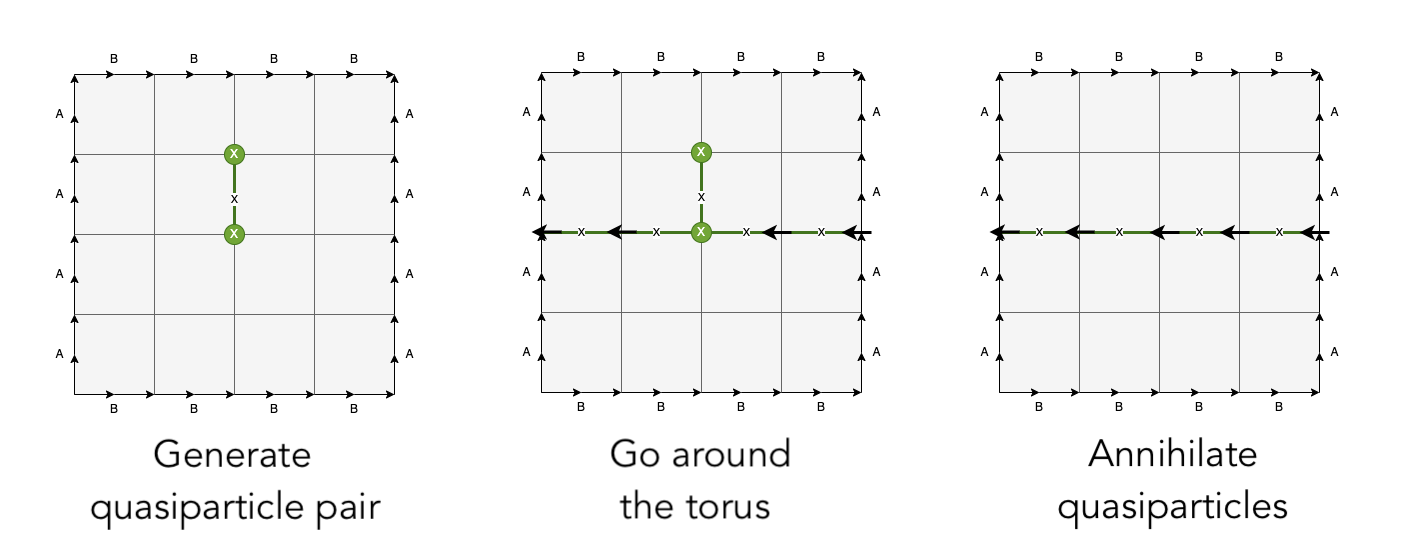
\includegraphics[scale=0.45]{not-alpha-gate}
\caption{Topological quantum process implementing the $\text{NOT}_{\alpha}$ gate}
\label{fig:not-alpha-gate}
\end{center}
\end{figure}

A diagram visualizing the process described in the following proposition is shown in Figure \ref{fig:not-alpha-gate}.

\begin{proposition} The following computation has the effect of performing the $\text{NOT}_{\alpha}$ gate. First, generate a particle/antiparticle pair of $X$-type particles. Then, move one of the particles around the torus via a path homologous to $\alpha$. Finally, fuse your two adjacent $X$-type particles together.
\end{proposition}
\begin{proof} Let $v_0$ and $v_1$ be adjacent vertices. Let $\alpha_0$ be a cycle homologous to $\alpha$ going from $v_1$ to itself. The process described in the statement of the proposition can be reworded as saying the following. First, we create a particle pair at $v_0$ and $v_1$, i.e, we tensor with $\sigma_X$ at the edge connecting $v_0$ and $v_1$. Then we move $v_1$ along $\alpha_0$, i.e, we tensor with $\sigma_X$ along the edges in $\alpha_0$. Then, we fuse the $X$-type quasiparticles at $v_0$ and $v_1$ back together, i.e, we tensor along the edge connecting $v_0$ and $v_1$ again. Since $\sigma_X^2=1$, this whole process can be described mathematically as

$$\bigotimes_{\text{edges in }\alpha_0}\sigma_X.$$

Seeing as $\sigma_X$s corresponds to flipping $\0$s to $\1$s in pure states, this process has the effect of flipping all of the qubits along $\alpha_0$. On the level of cycles, this means that we take $\left|\gamma\right>$ to $\left|\gamma+\alpha_0\right>$, where addition is in the group of cycles. Seeing as adding a cycle homologous to $\alpha$ to a cycle homologous to $\omega$ results in a cycle homologous to $\omega+\alpha$ we find thus that this process has the effect of sending $\left|\omega\right>$ to $\left|\omega+\alpha\right>$. Seeing as $\alpha+\alpha=0$ in $H_1(T;\ZZ_2)$, this process is exactly the $\text{NOT}_{\alpha}$ gate.
\end{proof}

Similarly, we can implement the $``(-1)_{\alpha}"$ gate, which flips the input state depending on whether it has an $\alpha$ component, namely

\begin{align*}
&\nullclass \mapsto \nullclass,\,\,  \betaclass \mapsto \betaclass \\
&\alphaclass \mapsto -\alphaclass,\,\, \alphabetaclass \mapsto -\alphabetaclass.
\end{align*}

\begin{proposition}\label{Xparticle} The following computation has the effect of performing the $\text{(-1)}_{\alpha}$ gate. First, generate a particle/antiparticle pair of $Z$-type particles. Then, move one of the particles around the torus via a path homologous to $\beta$. Finally, fuse your two adjacent $Z$-type particles together.
\end{proposition}
\begin{proof} Let $p_0$ and $p_1$ be adjacent faces. Let $\beta_0$ be a cycle homologous to $\beta$ going from $p_1$ to itself. Note that since $Z$-type particles live on faces, $\beta_0$ does not consist of a series of edges. Instead, it is a path going through the centers of faces. We take $\widehat{\beta}_0$ to be the set of edges that $\beta_0$ passes through. Tensoring with $\sigma_Z$ along $\widehat{\beta}_0$ corresponds to motion of a particle from $p_1$ along $\beta_0$ back to itself.

\begin{figure}
\begin{center}
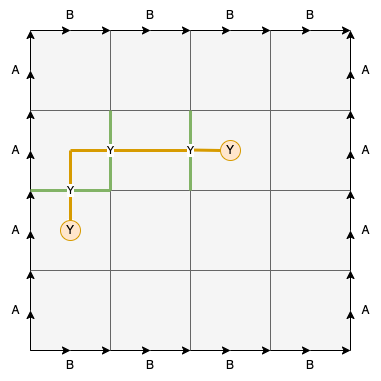
\includegraphics[scale=0.30]{dual-celluation}
\caption{Sample trajectory along dual celluation of torus}
\label{fig:dual-celluation}
\end{center}
\end{figure}

These cycles that go through faces of the torus are called \textit{dual cycles}, and are standard practice in the theory of homology. Namely, they are cycles in the dual celluation, as seen in Figure \ref{fig:dual-celluation}. Whereas the edges associated with a normal cycle satisfy the property `every vertex touches an even number of $1$s', the edges associated with a cycle in the dual celluation satisfy the dual condition `every face touches an even number of $1$s'.

As before, we find that the whole process can be described mathematically as

$$\bigotimes_{\text{edges in }\widehat{\beta}_0}\sigma_Z.$$

The matrix $\sigma_Z$ acts on pure states by sending $\0$ to itself, and $\1$ to $-\1$. Thus, this process has the effect of introducing a $-1$ global phase shift for every $1$ in states along $\widehat{\beta}_0$. Thus, when acting on a pure state $\gamma$, the definition of $\widehat{\beta}_0$ shows that this process has the effect of introduce a phase shift of $-1$ to the power of the number of intersection between $\gamma$ and $\widehat{\beta}_0$.

It is a well known fact that this signed intersection number ($-1$ to the power of the number of intersections) is an invariant in $\ZZ_2$ homology. To see this, observe that changing representatives of a homology class correspond to flipping qubits around a face. By the `dual cycle' condition, this flipped face will touch an even number of elements in the dual cycle. Hence, the intersection number will change by an even amount, leaving $-1$ to the power of that number invariant.

In particular, $\bold{0}$ doesn't intersect $\beta$, $\beta$ doesn't intersect $\beta$ (representatives can be chosen to be parallel), $\alpha$ intersects $\beta$ (horizontal loops and vertical loops meet at exactly one point), and $\alpha\beta$ intersects $\beta$. Thus, this process has the effect of adding a $-1$ phase shift to those states which include an `$\alpha$', as desired.
\end{proof}

Sadly for the toric codes, these are essentially the only gates that can be implemented. No matter how one moves around particles, there is not enough complexity in the system to generate interesting gates. We formalize this by writing out the \textit{group of gates} of the toric codes. We can think of quantum gates on a system as forming a group, where the group law is given by the composition of gates, and every element has an inverse since unitary matrices are invertible. For the toric codes, we have the following:

\begin{proposition}\label{Yparticle} There are exactly 8 possible computations in the toric codes. The group of gates is (non canonically) isomorphic to the Pauli group, i.e, the group whose objects are

$$\{\pm I, \pm iI, \pm \sigma_X, \pm i \sigma_X, \pm \sigma_Y, \pm i\sigma_Y, \pm \sigma_Z, \pm i \sigma_Z\}$$

and whose group operation is given by matrix multiplication. A minimal generating set is given by $\{\text{NOT}_{\alpha},\text{NOT}_{\beta},(-1)_{\alpha}\}$.
\end{proposition}
\begin{proof} To begin, we define $\text{NOT}_{\beta},\text{NOT}_{\alpha\beta},(-1)_{\beta},$ and $(-1)_{\alpha\beta}$ in complete analogy to how we define $\text{NOT}_{\alpha}$ and $(-1)_{\alpha}$. Namely, $\text{NOT}_{\beta}$ flips whether or not a state has a `$\beta$' in it, and $\text{NOT}_{\alpha\beta}$ flips whether or not a state has an `$\alpha\beta$' in it, i.e,

\begin{align*}
&\nullclass \mapsto \alphabetaclass,\,\,  \betaclass \mapsto \alphaclass \\
&\alphaclass \mapsto \betaclass,\,\, \alphabetaclass \mapsto \nullclass.
\end{align*}

The relation $\sigma_X\sigma_Z=-\sigma_Z\sigma_X$ implies that we can switch the order of operations between first applying all our $\sigma_X$s and then applying all our $\sigma_Z$s, up to an operator-wise phase shift $-1$. Any process of creating and annihilating $X$-type quasiparticles can be modeled in sequence as repeatedly creating particles, moving them around a loop, then annihilating them. Following the proof of Proposition \ref{Xparticle}, this is the same as repeatedly applying $\text{NOT}_{\omega}$ gates, for homology classes $\omega$. Similarly, the processes on $Z$-type particles will be compositions of $(-1)_{\omega}$ gates.

Hence, we now have a full set of generators for our gate group: $\{\pm I, \text{NOT}_{\omega}, (-1)_{\omega}\}$, where $\omega$ runs over homology classes. The relations $\text{NOT}_{\alpha}\text{NOT}_{\beta}=\text{NOT}_{\alpha\beta}$ and $(-1)_{\alpha}(-1)_{\beta}=(-1)_{\alpha\beta}$ allow one to reduce the generating set further. The relations

$$\text{NOT}_{\alpha}(-1)_{\alpha}\text{NOT}_{\alpha}=(-1)_{\beta}$$

and

$$(-1)_{\alpha}\text{NOT}_{\alpha}(-1)_{\alpha}=-I$$

reduce the generating set to $\{\text{NOT}_{\alpha},\text{NOT}_{\beta},(-1)_{\alpha}\}$. Verifying simple relations gates, it is simple to see that the gate group is isomorphic to the Pauli group, as desired.


\end{proof}


Before moving on to the next section, we make a few final remarks about the behavior of quasiparticles on the toric codes. Namely, we observe the following. Consider the full vector space $\Ncal$, and adjacent two adjacent $X$-type and $Z$-type quasiparticles. Consider the simple braiding of these particles around each other, as in Figure \ref{fig:braiding}. A line going under another corresponds to the particle having passed through that space first, before the other particle. This braiding can be obtained by first performing a twist halfway around the circle by $X$, then a twist all the way around the circle by $Z$, then finally moving the second half of the circle by $X$. This process corresponds to a transformation $\Ncal\to \Ncal$ (i.e, tensoring with the appropriate $\sigma_X$s and $\sigma_Z$s). The observation is that this transformation is \textit{not} the identity on the codespace. Namely, since $\sigma_Z\sigma_X=-\sigma_X\sigma_Z$, this operation corresponds to a global phase shift of $-1$ on the system.

Thus, the braiding of $X$ type and $Z$ type particles corresponds to a phase shift of $-1$. This is in contrast to braiding two identical $X$ type or $Z$ type particles, which corresponds to the identity since $\sigma_X$ and $\sigma_Z$ commute with themselves. All particles in the standard model of physics are \textit{fermions}, which give a phase shift of $-1$ when you braid them with themselves, or \textit{bosons}, which act by the identity when you braid them with themselves. Seeing as $X$ type and $Z$ type particles in the toric code braid by the identity with themselves, one would expect them to be bosons. However, bosons always braid by the identity with each other and hence the $-1$ phase shift from braiding $X$ and $Z$ type particles should be impossible. The conclusion is that these really are \textit{quasi}particles, which behave much differently than particles in the standard model. Quasiparticles with simultaneously non-bosonic and non-fermionic braiding rules are known as \textit{anyons}. All interesting particles in topological quantum phases of matter will be anyons.

In the case of the toric code, the braiding will always be trivial or give a global phase shift (i.e, -1). We call anyons \textit{non-abelian} if they can braid in such a way to create transformations that are not phase shifts. To  create interesting quantum gates, these sort of non-phase shift braidings are what we need. The search for a topological quantum computer is essentially the search for experimentally-sound easy-to-braid non-abelian anyons.

$\newline\newline$

\large \textbf{Exercises}:\normalsize

\begin{enumerate}[\thesection .1.]
\item For edges $v$ and faces $p$, define

$$A_v'=\bigotimes_{\substack{\text{edges} \\ \text{touching }v}}\sigma_X,\,\, B_p'=\bigotimes_{\substack{\text{edges} \\ \text{touching }p}}\sigma_Z,$$

$$H'=-\sum_{\text{vertices }v}A_v'-\sum_{\text{faces }p}B_p'.$$

Let $M=\frac{1}{\sqrt{2}}
\begin{pmatrix}
1 & 1 \\
1 & -1
\end{pmatrix}$ be the Hadamard matrix. Using the relations

$$\sigma_X=M\sigma_ZM^{-1},\,\, \sigma_{Z}=M\sigma_X M^{-1},$$

show that $H$ and $H'$ are similar, in the sense that $H'=MHM^{-1}$. Use this to conclude that all basis independent properties of the toric code are formally symmetric by replacing $X$ with $Z$. In particular, the codespace (lowest eigenspace) of $H'$ is 4 dimensional, and the gate group of $H'$.


\item Show that eigenvectors of the Hamiltonian are equally likely to give $0$ or $1$ when measured at every qubit [HINT: Prove this for ground states first, then lift to general eigenstates using an induction argument along the lines of the proof of Proposition \ref{eigenspaces}] [WORK: Does this imply that eigenvectors are maximally entangled?]

\item Let $\Ncal_{n}$ denote the vector space associated to the $n$ by $n$ grid on the torus. Let

$$\tilde{H}_n=H_n+(2n^2)I,$$

so that the ground states have eigenvalue $0$. This is more physically realistic, since systems cannot have negative energy. When $n$ divides $m$, we have a natural map

$$\Ncal_{n}\hookrightarrow{}\Ncal_{m}$$

defined by [WORK: What is the correct definition?]. Show that this map is linear and injective, and hence that $\Ncal_{n}$ can be realized as a sub vector space of $\Ncal_{m}$. Show that $\tilde{H}_{m}$ restricted to $\Ncal_{n}$ is equal to $\tilde{H}_n$. Show that the map $\Ncal_{n}\hookrightarrow{}\Ncal_{m}$ is norm-preserving, in the sense that if $\left|\chi\right>,\left|\psi\right>$ are states on $\Ncal_{n}$, the inner product $\left<\chi | \psi \right>$ is independent of whether or not it was computed in $\Ncal_{n}$ or $\Ncal_{m}$. Define

$$\Ncal_{\infty}=\bigcup_{n=3}^{\infty}\Ncal_{n},$$

and define $\tilde{H}_{\infty}$ to be the operator on $\Ncal_{\infty}$ which acts on vectors in $\Ncal_{n}$ by $\tilde{H}_n$. Show that these are well defined objects, that $\Ncal_{\infty}$ is naturally a Hilbert space. It is in this sense that we can speak of a limiting continuous model formed by the discrete grid celluations.
\footnote{Note that objects in $\Ncal_{\infty}$ themselves aren't continuous paths; they are just discrete cycles in $\Ncal_n$ for some $n$. This is not an issue, since the \textit{simplicial approximation theorem} says that every continuous phenomenon can be modeled discreetly in a fine enough celluation.}
\end{enumerate}

\section{Topological Quantum Field Theories}
\label{TQFTs}

\subsection{The general picture}

Topological Quantum Computation (TQC) is physically based on topological quantum phases of matter. Topological Quantum Field Theories are the mathematical formalism of topological quantum phases of matter. Namely, every topological quantum phase of matter (physical object) has an associated Topolgoical Quantum Field Theory (mathematical object) to describe it. To make this clearer, we recall classical phases of matter in a more mathematically rigorous way. Namely, a phase of matter is an assignment

$$
\begin{pmatrix}
\text{Collections of } \\
\text{particles}
\end{pmatrix}
\bigleadsto
\begin{pmatrix}
\text{Physical\,} \\ \text{systems}
\end{pmatrix},
$$

taking a set of particles to the way it would behave under the phase of matter. The ``gas" phase of matter will take a collection of particles and make the physical system of having them all bounce around each other really fast. The ``solid" phase of matter will take that same collection of particles and have them move less freely, and form a more cystalline structure. A quantum phase of matter should do the exact same thing, but now your physical system is a quantum system. Namely, a quantum phase of matter is an assignment

$$
\begin{pmatrix}
\text{Collections of } \\
\text{particles}
\end{pmatrix}
\bigleadsto
\begin{pmatrix}
\text{Quantum\,} \\ \text{systems}
\end{pmatrix}.
$$

Topological quantum phases of matter arrise from the understanding that the topology of a shape (i.e, the physical invariants of the shape invariant up to deformation) will effect the quantum system arrising from inducing that shape with a given phase of matter. For example, we consider the ``$\ZZ_2$ spin liquid" topological quantum phase of matter, described in the introduction. When this phase of matter is induced a torus, the resulting quantum system will always be four dimensional (Proposition \ref{eigenspaces}). If the $\ZZ_2$ spin liquid is induced on the torus with two holes (see Figure \ref{fig:genus-two}), the ground space will instead be sixteen dimensional. Thus, a topological quantum phase of matter is an assignment

\begin{figure}
\begin{center}
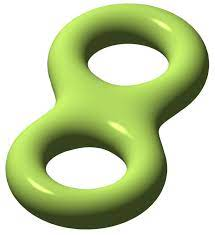
\includegraphics[scale=0.25]{genus-two}
\caption{The two holed torus (surface of genus of 2)}
\label{fig:genus-two}
\end{center}
\end{figure}

$$
\begin{pmatrix}
\text{Topological } \\
\text{spaces}
\end{pmatrix}
\bigleadsto
\begin{pmatrix}
\text{Quantum\,} \\ \text{systems}
\end{pmatrix}.
$$

All of the interesting quantum systems are on two dimensional spaces. This can be seen as follows. TQC is performed by braiding quasiparticles through spacetime. When space is two dimensional, spacetime is three dimensional. When space is three dimensional, spacetime is four dimensional. It is a theorem that there are no knots in four dimensions: The extra dimension gives the knot room to move around and untangle. Thus, to have nontrivial knots, space must be two dimensional. A two dimensional space is called a \textit{surface}. The surfaces we are interested in are those two dimensional spaces which can be embedded into three dimensional space, i.e, those surfaces which can be realized physically in our three dimensional world. Note that there are some weird surfaces which can not be embedded into three dimensional space, such as the Klein bottle (shown in Figure  \ref{fig:klein-bottle}). While the `true' surface does not intersect itself, any way of placing it in three dimensions will self intersect. One needs an extra dimension to avoid this intersection.

\begin{figure}
\begin{center}
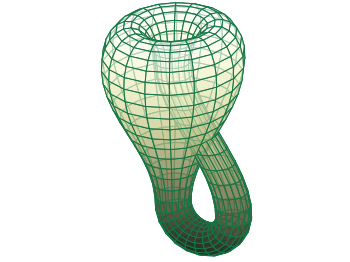
\includegraphics[scale=0.25]{klein-bottle}
\caption{The Klein bottle, attempting to be embedded in 3d space}
\label{fig:klein-bottle}
\end{center}
\end{figure}

This condition on embeddability into three dimensional space makes our study of surfaces much simpler. Namely we have the following well-known theorem from topology:

\begin{theorem} Consider a surface that

\begin{enumerate}
\item Is finite in area (for example, an infinitely stretched flat plane would not count)
\item Has no boundary (for example, a unit disk would not count, since its boundary is the circle)
\item  Can be embedded intro three dimensional space.
\end{enumerate}

Then, this surface must be a collection of $g$-holed torii, for some integers $g\geq 0$.
\end{theorem}

Thus, going forward the word `surface' will simply refer to a collection of $g$-holed torii. A connected surface is one which can not be decomposed as the union of two other smaller surfaces. Every connected surface will be the $g$-holed torus for some $g\geq0$, and more general surfaces can all be uniquely written as a union of connected surfaces. A two dimensional topological quantum phase of matter is thus an assignment

$$
\begin{pmatrix}
\text{Surfaces} \\
\text{in space}
\end{pmatrix}
\bigleadsto
\begin{pmatrix}
\text{Quantum\,} \\ \text{systems}
\end{pmatrix}.
$$

Concretely, we refer to the $g$-holed torus as $T_g$. Mathematically, a quantum system is complex vector space. Hence, a topological quantum phase of matter is an assignment

$$S \,\mathlarger{\leadsto}\,V(S)$$

for each surface $S$, where $V(S)$ is a finite dimensional vector space over the complex numbers. This mathematical formalism is known as Topological Quantum Field Theory. Namely, the assignment $S \,\mathlarger{\leadsto}\,V(S)$, \textit{is} a Topological Quantum Field Theory. To ease terminology, we will from now on use the abbreviation TQFT.

Not every assignment of surfaces to vector spaces will be a TQFT. Namely, many will be `un physical', meaning that they never could have come from topological phases of matter. For example, the axioms of quantum mechanics say that putting two quantum systems together should correspond to the tensor product of those two systems. Formally, we should have

$$V\left(S_0\sqcup S_1\right)=S_0\otimes S_1.$$

Here, $\sqcup$ denotes the disjoint union. The disjoint union is the same as a union, but it specifies that the union should be taken in a way such that $S_0$ and $S_1$ do not intersect (i.e, that they are disjoint). The disjoint union can be intuitively read as simply putting two spaces next to each other.

Additionally, by the axioms of quantum mechanics, transformations of a surface through spacetime should correspond to linear (unitary!) maps on quantum systems. We think mathematically about what a trajectory through spacetime looks like. In the one dimensional case, suppose we have two particles $a$ and $b$. A trajectory through spacetime from $a$ to $b$ is a path $e$ connecting $a$ and $b$. Thinking deeply, one observes that the condition of ``connecting" $a$ and $b$ can be mathematically stated as $\partial e= a \sqcup b$, where $\partial e$ denotes the boundary of $e$. This is shown in Figure \ref{fig:bordism}.

\begin{figure}
\begin{center}
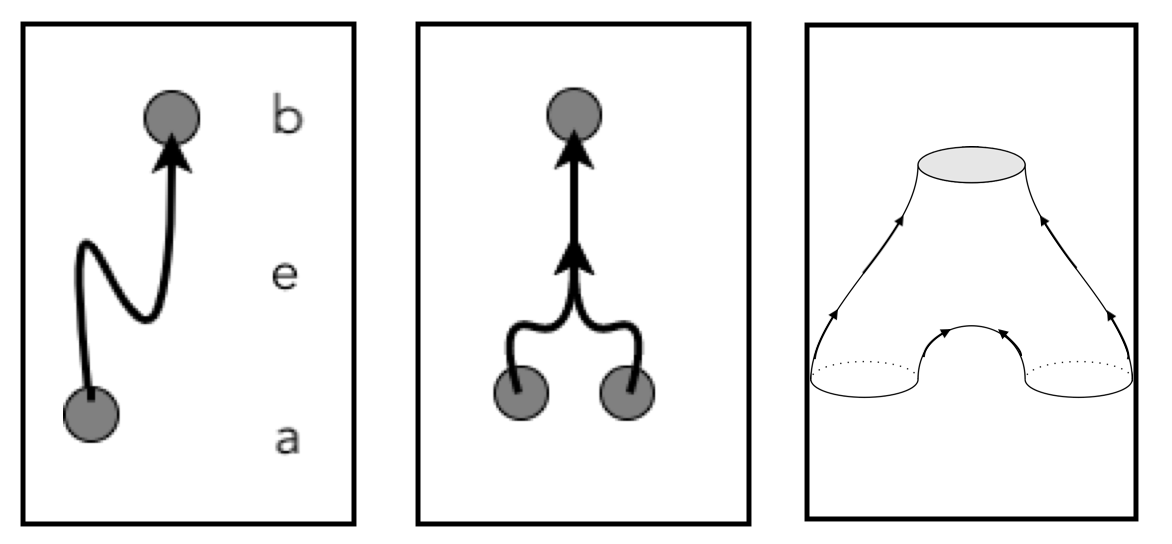
\includegraphics[scale=0.40]{cobordism}
\caption{First box - A path in spacetime from $a$ to $b$ by $e$, i.e, a path $e$ with $\partial e= a \sqcup b$. Second box - The fusion of two particles in spacetime. Third box - the fusion of two circles in spacetime, known informally as a ``Pair of Pants".}
\label{fig:bordism}
\end{center}
\end{figure}

We observe however an ambiguity: Time has direction, but our edge does not. Hence, it is impossible to distinguish a path from $a$ to $b$ and a path from $b$ to $a$. For this reason we have to introduce the concept of \textit{orientation}. An oriented path is a path with a choice of direction. This can be visualized by putting a consistent set of arrows on the path. The points that the edge is going away from correspond to the particles at the beginning of some process, and the points at the end correspond to the particles at the end of that process. Note that the paths can join and split, as seen in the second box of Figure  \ref{fig:bordism}. This corresponds to the fusion and anihilation of particles. Given two circles,

We now try to generalize this picture to the case of surfaces. Remember, our goal is to mathematically describe a trajectory of surfaces through spacetime, which will be key to our theory since these will correspond to linear transofrmations on the quantum system. The key insight is as follows. Given two sets of $A$ and $B$ (still representing particles), we saw a trajectory through spacetime was a path $E$ such that $\partial E=A\sqcup B$. Let $A$ and $B$ be two circles, or unions of circles, a trajectory through spacetime is a surface (with boundary, namely, not neccecary a torus) $E$ such that $\partial E = A\sqcup B$, just as in the third box of \ref{fig:bordism}. Given two surfaces $S_0$ and $S_1$ (with no boundary, as usual), a trajectory through spacetime should be a three dimensional object $X$ whose boundary is $\partial X= S_0\sqcup S_1$.

Defining what we mean exactly by three dimensional object is very technical. Namely, these objects should be $3$-manifolds, in the same way that a surface is a $2$-manifold, a path is a $1$-manifold, and a set of points is a $0$-manifold. An introduction to the theory of manifolds can be found in Spivak's textbook \cite{spivak2018calculus}. We leave the notion vague. One can think of three manifolds as being filled in shapes. For instance, the torus is a surface ($2$-manifold), but the filled in solid torus is a $3$-manifold. Let $X$ be the solid torus with a smaller torus removed from inside it. Then the boundary $\partial X$ will be equal to the disjoint union of the outside torus and the smaller inside torus. We can see that $X$ forms a trajectory through spacetime, as the bigger torus contracts onto the smaller one. Again, though there is an ambiguity. How do we know that $X$ is a contraction big to small? Instead, it could have been an expansion small to big. To fix this issue, we will again have to speak of oriented $3$-manifolds. This gives every region on the $3$-manifold a direction: Imagine a series of areas inside of $X$ all pointing outside from the direction of the small inside torus toward the direction of the larger outside torus.

We introduce a piece of notation. When $\partial X = S_0 \sqcup S_1$ is the disjoint union of two surfaces, one of those surfaces (say, $S_0$) will always be the stuff going in, and one of those surfaces (say, $S_1$) will always be the stuff going on. We put this in the notation as $\partial X = (-S_0)\sqcup S_1$, to make inputs/outputs clearer. This mathematical formalism of a trajectory through spacetime is called a \textit{bordism}\footnote{Sometimes called a cobordism; the difference is immaterial.}. Namely, a bordism from a surface $S_0$ to a surface $S_1$ is a $3$-manifold $X$ such that $\partial X = (-S_0)\sqcup S_1$. With this out of the way, we can formally define a TQFT:

\begin{definition}[$(2+1)$-TQFT] A $(2+1)$ Topological Quantum Field Theory (TQFT) is the following data.
\begin{enumerate}
\item A choice of finite dimensional complex vector space $V(S)$ for every surface $S$.
\item A choice of linear transformation $Z(X): S_0\xrightarrow{} S_1$ for every bordism $X$ from $S_0$ to $S_1$.
\end{enumerate}
Additionally, a $(2+1)$-TQFT is required to satisfy the following compatibility properties:
\begin{enumerate}
\item (Union = tensor product). $V(S_0\sqcup S_1)=V(S_0)\otimes V(S_1)$. Here, $S_0$ and $S_1$ are any two surfaces.
\item (Composing processes = composing transformations). $Z(X'\cup X)=Z(X')\circ Z(X)$. Here, $X$ is a bordism from two surfaces $S_0$ and $S_1$, and $X'$ is a bordism from surfaces $S_1$ to $S_2$. One easily verifies that their union is a bordism between $S_0$ and $S_2$, whose induced map we can compare with the composition of the induced maps of $X$ and $X'$.

\item (Swap spaces = swap tensor factors) The linear map associated with the bordism $X$ from $S_0\sqcup S_1$ to $S_1\sqcup S_0$ defined by taking $S_0,S_1$ and moving them around each other correspond to the linear map $V(S_0)\otimes V(S_1)\xrightarrow{} V(S_1)\otimes V(S_0)$ defined by sending $v\otimes w$ to $w\otimes v$.
\item (Time reversal symmetry) [WORK: Find concise way to word this without having to consider oriented surfaces]
\item .[WORK: What are the other axioms?] This completes the definition.
\end{enumerate}
\end{definition}

We offer a few remarks. The term ``$(2+1)$" refers to the fact that there are two spaces dimensions, plus one time dimension. More generally, an  $(n+1)$-TQFT is an assignment of $n$-manifolds to vector spaces, and of $(n+1)$-manifolds to linear transformations. We also remark on the structure of the definition. We first define a few assignments of objects of one type to objects of another type, and then we define a laundry list of properties that those assignments should satisfy. This is extremely standard practice in higher mathematics. The abstraction of this practice is known as Category Theory. The assignments of one type of object to another type of object are known as functors, and the properties to satisfy are known as axioms. The category theory definition of a TQFT is ``A symmetric monoidal functor from the category of bordisms to the category of vector spaces". For those unfamiliar with category theory, a short introduction is found in Appendix \ref{Categories}. While we will not be using any category theory in this section, a familiarity of the subject is required for the following section on Modular Tensor Categories.

\subsection{The $\ZZ_2$ Dijkgraaf-Witten TQFT}

We now define the Topological Quantum Field Theory (TQFT) assoicated with the toric code, and describe how TQC can be performed in this framework. We could also call this the ``$\ZZ_2$ spin liquid TQFT", since that is the topologcial quantum phase of matter which physically realizes the $\ZZ_2$ spin liquid topological quantum phase of matter.

As with the definition of the toric codes in Section \ref{The Toric Code}, the definition of the $\ZZ_2$ Dijkgraaf-Witten TQFT is in the language of $\ZZ_2$ homology. Seeing as our definition of homology requires a celluation we first define $\tilde{V}(S,\Delta)$, where $S$ is a surface and $\Delta_S$ is a celluation of $S$. That is, $\Delta_S$ is a representation of $S$ as a collection of verticies, edges, and faces, with some edges and verticies identitied. For example, $S=T$ could be the torus, and $\Delta$ could be the $n$ by $n$ lattice on the torus. For every surface $S$ and celluation $\Delta_S$, we define

$$\tilde{V}(S,\Delta_S)=\CC\left[C^{1}(\Delta_S;\ZZ_2)\right].$$

Here, $C^1(\Delta_S;\ZZ_2)$ denotes the group $\ZZ_2$ cocycles on the celluation $\Delta_S$, and $\CC[-]$ is notation for ``complex vector space generated by", i.e, $\tilde{V}(S)$ is the unique complex vector space having $C^1(\Delta_S;\ZZ_2)$ as a basis. A $\ZZ_2$ cocycle is an assignment of $0$s and $1$s to every edge, such that every face touches and even number of $1$-labeled edges.

Notice that a $\ZZ_2$ cocycle is the same thing as a $\ZZ_2$ cycle in the dual celluation, as discussed in the proof of Proposition \ref{Xparticle}. That is, every $\ZZ_2$ cocycle on $S$ specifies a cycle on $S$, by drawing lines between the centers of two faces whenever the edge connecting them is labeled by a $1$. This process of identifying cocycles on $\Delta_S$ and cycle in the dual celluation is known as Poincaré Duality. It is important to note that in higher dimensions the process breaks down, because generically loops will fail to intersect in three dimensions (they can just be shifted past each other). Thus, when discussing 3-manifold bordisms there is a real distinction between cycles and cocycles.

The reason we call this $\tilde{V}$ instead of $V$ is that it depends on the choice of celluation $\Delta_S$, and we want $V(S)$ to only depend on $S$. The invariant subspace $V(S)$ is defined like so:

$$V(S)=\CC[H^1(S;\ZZ_2)],$$

where $H^1(S;\ZZ_2)$ is the cohomology of $S$. Cohomology is defined by

$$H^1(S;\ZZ_2)=C^1(S;\ZZ_2)/Z^1(S;\ZZ_2),$$

where $Z^1(S;\ZZ_2)$ is the subgroup of of $C^1(S;\ZZ_2)$ generated by the cocycles consisting of $1$s at every edge touching a vertex. Assigning $1$s and $0$s this way really does give a cocycle: Every face has either $0$ or $2$ edges in its boundary that touch a given vertex, and both $0$ and $2$ are even numbers. It is a standard fact that the cohomology of a space does not depend on the choice of celluation.

To view $V(S)$ and a subspace of $\tilde{V}(S,\Delta_S)$, we define a linear injection

\begin{align*}
V(S)&\hookrightarrow \tilde{V}(S,\Delta_S).\\
\left|\alpha\right>&\mapsto \frac{1}{|Z^1(S;\ZZ_2)|}\sum_{\gamma\sim \alpha}\left|\gamma\right>
\end{align*}

Here, $\alpha$ is a cohomology class (an element of $H^1(S;\ZZ_2)$), $\left|\alpha\right>$ is the corresponding vector in $V(S)$, $|Z^1(S;\ZZ_2)|$ denotes the number of elements in $Z^1(S;\ZZ_2)$, and $\sim$ denotes the equivilance relation of being cohomologous. That is, two cocycles are cohomologous if they give the same element in $H^1(S;\ZZ_2)$. This map can be summarized by saying that a cohomology class sends to the equal superposition of all of its representatives. The normalizing factor $|Z^1(S;\ZZ_2)|^{-1}$ is introduced to make sure that the norm is preserved.

We now define the action of bordisms. Let $(S_0,\Delta_{S_0})$ and $(S_1,\Delta_{S_1})$ be two surfaces with celluations. Let $X$ be a bordism from $S_0$ to $S_1$. Let $\Delta_X$ be a celluation on $X$ compatible with the celluations on $S_0$ and $S_1$. By compatible we mean that if we restrict $\Delta_X$ to $\partial X$ then we will recover the celluations $\Delta_{S_0}$ and $\Delta_{S_1}$. This restriction process can be described visually as dropping all verticies, edges, and faces, from $\Delta_X$ that aren't part of $\partial X=S_0\sqcup S_1$. We call a pair of cocycles $(\omega_{S_0},\omega_{S_1})$ extendable if there is a cocycle in $\omega_X\in C^1(X,\Delta)$ which gives $\omega_{S_0}$ when restricted to $S_0$ and $\omega_{S_1}$ when restricted to $S_1$. This allows us to put

$$\tilde{Z}(X,\Delta_X)=\begin{pmatrix}
$1$\text{ if }(\omega_{S_0},\omega_{S_1})\text{ extendable}\\
$0$\text{ otherwise }
\end{pmatrix}_{\substack{\omega_{S_0}\in C^1(S_0;\ZZ_2) \\ \omega_{S_1}\in C^1(S_1;\ZZ_2)}}.$$

We elaborate on the meaning of this expression. Linear algebra tells us that to specify a linear transformation between two spaces, all we need to do is specify the entries of a matrix. The entries of a matrix are labeled by basis vectors. Namely, for a map $\CC[C^1(S_0;\ZZ_2)]$ to $\CC[C^1(S_1;\ZZ_2)]$ the entries of the matrix are labeled by ordered pairs of basis vectors $(\left|\omega_{S_0}\right>,\left|\omega_{S_1}\right>)$, where $\omega_{S_0}\in C^1(S_0;\ZZ_2)$ and $\omega_{S_1}\in C^1(S_1;\ZZ_2)$. The $(\omega_{S_0},\omega_{S_1})$ entry in $\tilde{Z}(X;\Delta_X)$ is equal to $1$ if $(\omega_{S_0},\omega_{S_1})$ is extendable, and $0$ otherwise.

The intuitition for $\tilde{Z}(X,\Delta_X)$ comes from the path integral formulation of quantum mechanics. When not being observed, a system will transform along a superposition of all possible trajectories. There is a spacetime trajectory from a state  (cocycle) $\left|\omega_{S_0}\right>$ to a state (cocycle) $\left|\omega_{S_1}\right>$ exactly when $(\omega_{S_0},\omega_{S_1})$ can be extended. The map $\tilde{Z}(X,\Delta_X)$ can be described as the transformation that takes a state to the equal superposition of all possible states it could go to.

Our goal is to show that $\tilde{Z}(X,\Delta_{X})$ restricts to a map $V(S_0)\xrightarrow{}V(S_1)$, and that this restriction is independent of our choice of $\Delta_{S_0}, \Delta_{S_1}$ and $\Delta_{X}$. Once this has been done we can define $Z(X)$ to be this common restriction. All that will be left to do then is to show that our assignments $V(S)$ and $Z(X)$ satisfy the axioms of a $(2+1)$-TQFT. We work on this overarching plan over the course of a few propositions.

\begin{proposition} Let $(S_0,\Delta_{S_0})$ and $\left(S_1,\Delta_{S_1}\right)$ be surfaces with celluations, $X$ a bordism from $S_0$ to $S_1$, and $\Delta_X$ a celluation of $X$ compatible with the celluations on $S_0$ and $S_1$. Then, the map $\tilde{Z}(X,\Delta_X): \tilde{V}(S_0,\Delta_{S_0})\xrightarrow{}\tilde{V}(S_1,\Delta_{S_1})$ is independent of the choice of celluation $\Delta_X$. Hence, we can properly omit $\Delta_X$ from our notation, and speak of a well defined map $\tilde{Z}(X)$.
\end{proposition}
\begin{proof}
.[WORK: Understand Turaev-Viro's approach, and reference it here] We reference \cite{turaev1992state} for Tureav-Viro's work, and \cite{lickorish1999simplicial} for a readable survey. Figure \ref{fig:moves} should show the relevant moves.
\end{proof}

\begin{figure}
\begin{center}
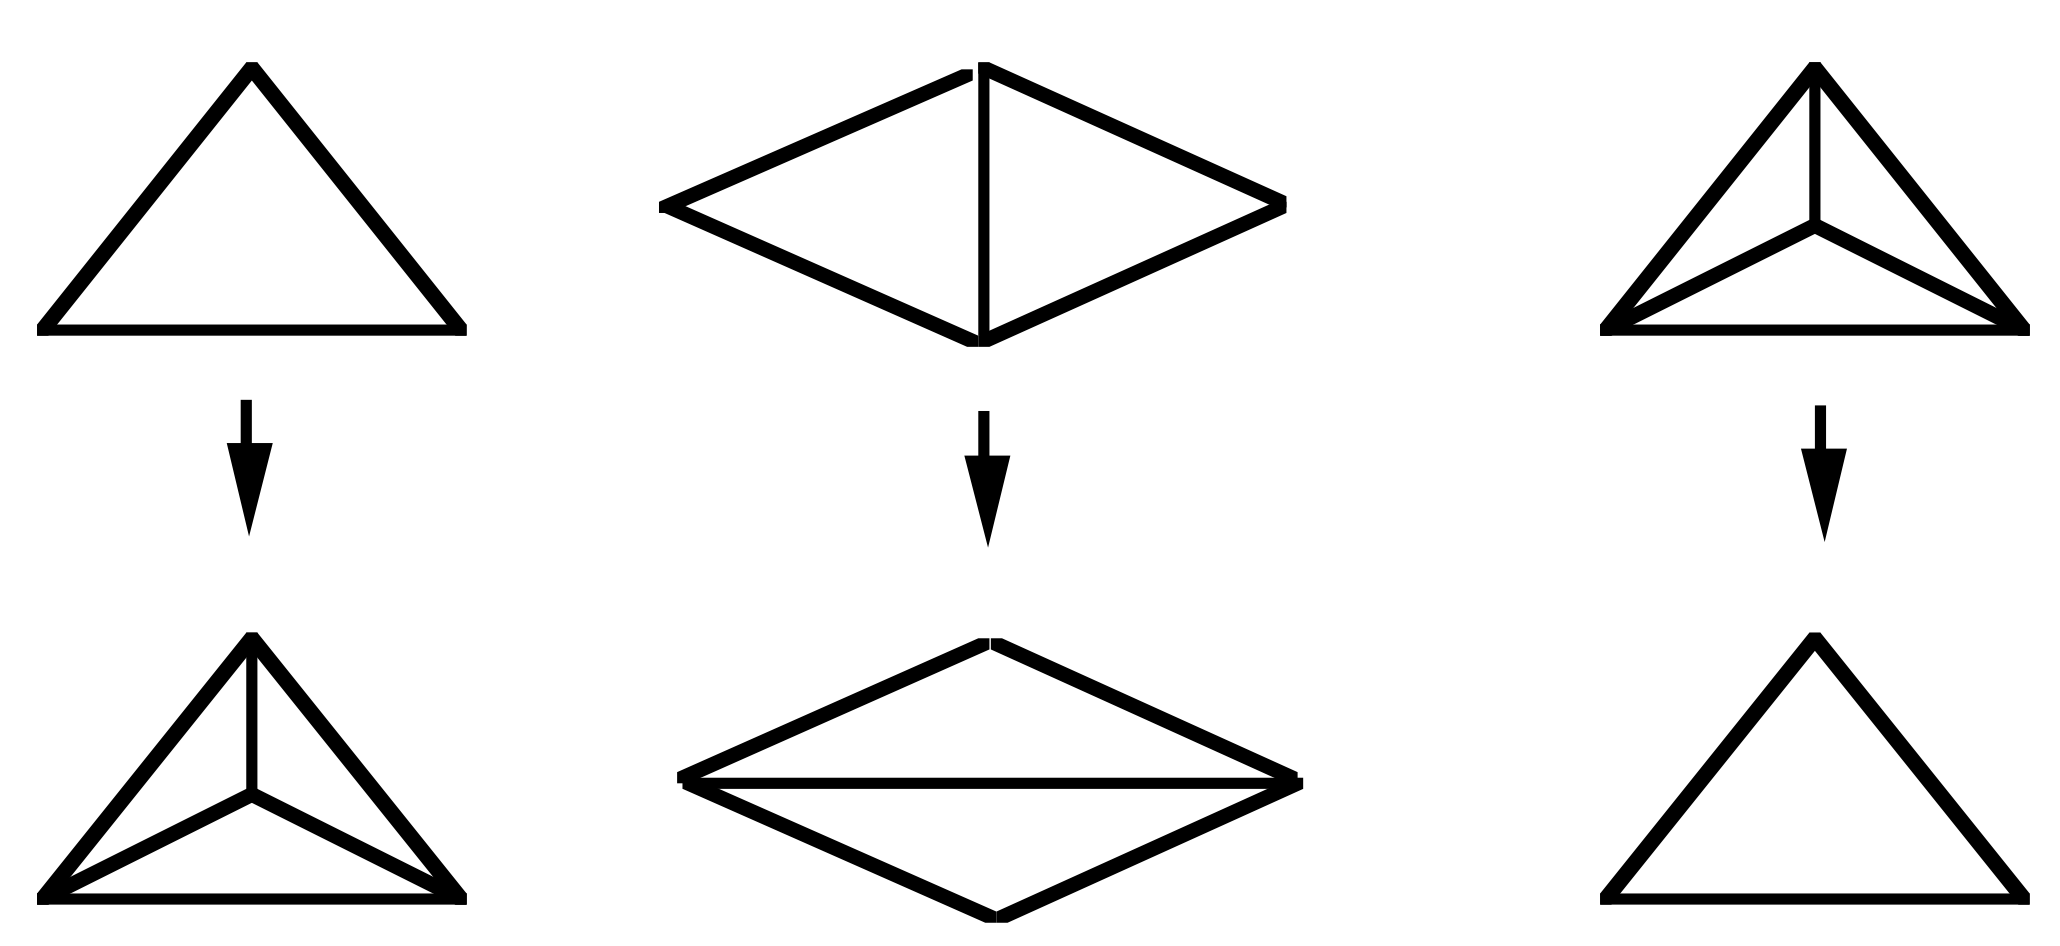
\includegraphics[scale=0.15]{moves}
\caption{Full set of moves for going from any simplicial complex to any other simplicial complex}
\label{fig:moves}
\end{center}
\end{figure}

\begin{proposition} Let $(S_0,\Delta_{S_0})$, $(S_1,\Delta_{S_1})$, $(S_1,\Delta_{S_2})$ be surfaces with celluations, let $X$ be a bordism from $S_0$ to $S_1$, and let $X'$ be a bordism from $S_1$ to $S_2$. The composition law

$$Z(X'\cup X)=Z(X')\circ Z(X)$$

holds.
\end{proposition}
\begin{proof} Consider a celluation $\Delta_{X'\cup X}$ on $X'\cup X$, which is simultaneously compatible with $\Delta_{S_0}$, $\Delta_{S_1}$, and $\Delta_{S_2}$. [WORK: Should I add a reference to the fact that you can always choose these liftings?]. [WORK: We need good scaling factors to make this work]
\end{proof}

The next proposition has a strong physical meaning, and can be seen as motivation for the fact that $V(S)$ is a ground state space. Namely, let $(S,\Delta_S)$ be a surface with celluation and let $S\times [0,1]$ be the product of $S$ with the real interval of numbers between $0$ and $1$. That is, elements of $S\times [0,1]$ are pairs $(s,t)$ where $s\in S$ and $t\in [0,1]$. This is a $3$-manifold, and gives a bordism from $S$ to itself. Namely, $\partial (S\times [0,1])$ is built of the two components $S\times \{0\}$ and $S\times \{1\}$. The orientation on $S\times [0,1]$ is induced by the orienation on $[0,1]$. This can viewed as the identity bordism: $S$ is doing nothing as time increases from $0$ to $1$. The boundary components correspond to the placement of $S$ at time $0$ and $S$ at time $1$. When time passes on a system, we expect it to ambiently decrease in energy. Thus,  physically $Z(S\times [0,1])$ should act by the identity on ground states, and send higher energy states down to the ground state. This is exactly the statement that $Z(S\times [0,1])$ should be a projection from the full state space to the ground state space. The following proposition in this lens thus says that $V(S)$ are exactly the ground space:

\begin{proposition} Let $(S,\Delta_S)$ be a surface with celluation. Viewing $S\times [0,1]$ as a bordism from $S$ to itself, we have that $\tilde{Z}(S\times [0,1])$ is a projection from $\tilde{V}(S,\Delta_S)$ to $V(S)$. Namely, the image of $\tilde{Z}(S\times [0,1])$ is $V(S)$, and $\tilde{Z}(S\times [0,1])$ acts by the identity on $V(S)$. Explicitely, $\tilde{Z}(S\times [0,1])$ is given by the map

$$\left| \omega\right>\mapsto \frac{1}{\sqrt{\# \text{ cohomologus things}}}\sum_{\gamma \sim \omega}\left|\gamma\right>$$

[WORK: Find the correct statement]
\end{proposition}
\begin{proof}. [WORK: Choose the good celluation and prove by flipping one at a time.]
\end{proof}

This allows us to prove the full idependence of our theory from arbitrary choices of celluations:

\begin{proposition} Let $(S_0,\Delta_{S_0})$ and $\left(S_1,\Delta_{S_1}\right)$ be surfaces with celluations, and $X$ a bordism from $S_0$ to $S_1$. The image of $\tilde{Z}(X)$ is contained in $V(S_1)$. In particular, $\tilde{Z}$ restricts to a map $V(S_0)\xrightarrow{}V(S_1)$. This map is independent of our choice of $\Delta_{S_0}$ and $\Delta_{S_1}$. We define $Z(X): V(S_0)\xrightarrow{}V(S_1)$ to be this common restriction.
\end{proposition}
\begin{proof} .[WORK: Find proof. I think this might trivially follow from postcomposing $X$ with $S_1\times I$, which acts trivally on $X$, and by independence of maps from celluations this should give the correct answer.]
\end{proof}

The main result of our section is as follows:

\begin{theorem} The assignments $S\mapsto V(S)$ and $X\mapsto Z(X)$ give a Topological Quantum Field Theory, called the $\ZZ_2$ Dijkgraaf-Witten TQFT.
\end{theorem}
\begin{proof}. [WORK: Find proof]
\end{proof}

\subsection{TQC with Dehn twists}


\section{Modular Tensor Categories}
[WORK: Make section]

\section{The Big Picture}
[WORK: Make section]


\appendix

\section{$\ZZ_2$ Homology Theory}
\label{Homology}

In this appendix we introduce the basic notations of homology theory with $\ZZ_2$ coefficients, namely, chains, cycles, and homological equivalence. The settings for homology are \textit{simplicial complexes}, which can be loosely thought of as collections of vertices, edges, and faces, with some edges and vertices identified, just as was done for the torus in this text. A $\ZZ_2$-chain on a space is an assignment of an element of $\ZZ_2$ to every edge, where $\ZZ_2=\{0,1\}$ is the additive group modulo 2. The set of $\ZZ_2$-chains forms a group under edge-wise addition. A $\ZZ_2$-cycle is a $\ZZ_2$-chain which can be obtained by starting at a vertex and walking along edges, flipping $1$s to $0$s and vice versa as you go along, and returning back where you started at the end. Equivalently, a $\ZZ_2$-cycle is a $\ZZ_2$-chain which has an even number of $1$s touching each vertex. The $\ZZ_2$-cycles form a subgroup of the group of $\ZZ_2$-chains. Seeing as all chains and cycles discussed in these notes take coefficients in $\ZZ_2$, we ease notation by simply saying ``chain" and ``cycle".

The goal of homology theory is to describe cycles on a geometric object, up to deformations. If one cycle can be continuously deformed into another, then they should be considered equivalent. On the sphere, for example, all loops can be contracted away into nothing. On the torus there are four distinct cycles, namely, the zero cycle, the cycle that goes around the torus horizontally, the cycle that goes around the torus vertically, and the cycle that twists around the torus, as in Figure \ref{fig:homology} These non-trivial cycles correspond exactly to the continuous vector fields described in the introduction \cite{frankel1957homology}.

Loosely, we will call two cycles homologically equivalent if they can be continuously deformed one to another. Given any face, the cycle consisting of $1$s along the edges touching that face should be `homologically trivial", i.e, homologically equivalent to the $0$ cycle, since it can be contracted away into nothingness. In a strong sense, this is the only condition one needs to impose. WIth $X$ as our simplicial complex, we let $C_1(X;\ZZ_2)$ be the group of chains. We let $Z_1(X;\ZZ_2)$ be the subgroup generated by the cycles consisting of $1$s  the boundaries of faces. This is the subgroup of homologically trivial cycles. This lets us define the quotient

$$H_1(X;\ZZ_2)=C_1(X;\ZZ_2)/Z_1(X;\ZZ_2),$$

called the ($1$st) homology group of $X$. Two elements are called homologically equivalent if they are in the same coset of $H_1(X;\ZZ_2)$. Alternatively, two elements are homologically equivalent if one can be obtained from the other by repeatedly flipping $1$s and $0$s along the boundaries of squares.

It is a well known fact that the first homology group of the torus has four elements, corresponding to the zero class, the horizontal cycle around the torus, the vertical cycle around the torus, and the diagonal cycle.

The importance of $H_1(X;\ZZ_2)$ is that it is \textit{independent of choice of celluation}. Namely, if we start with the same space and chop it up into verticies, edges, and faces, two different ways, $H_1(X;\ZZ_2)$ will always be the same. This is in stark contrast to $C_1(X;\ZZ_2)$ and $Z_1(X;\ZZ_2)$, which will both change wildly depending on the choice of celluation.

The observant reader might find the above discussion frustrating. In particular, we seem to be using the following intuitions interchangeably:

\begin{enumerate}
\item Cycles being continuously deformed to each other
\item Cycles that can be obtained from one another by flipping edges along the boundary of faces.
\end{enumerate}

The worry regarding the distinction between these two notions is justified. In general, the group obtained by imposing the equivalence relation of continuous deformations will not be equal to the homology group $H_1(X)$. The group resulting from imposing the continuous deformation restriction is called the \textit{fundamental group} of $X$, and is denoted $\pi_1(X)$. In general $\pi_1(X)$ can be quite a bit larger than $H_1(X)$, i.e, the equivalence relation can be weaker. The groups are always related by the fact that $H_1(X)$ is canonically isomorphic to the abelianization of $\pi_1(X)$, i.e, the maximal abelian quotient of $H_1(X)$. In the case that $\pi_1(X)$ is abelian (for example, when $X$ is a torus), this means that there is no distinction between these spaces, and one should not make any worry about the discrepancies in intuition.

The canonical reference for this subject (known as \textit{Algebraic Topology}) is Alan Hatcher's textbook \cite{hatcher2005algebraic}.

\section{Category Theory}
\label{Categories}
[WORK: Make appendix]

\bibliographystyle{alpha}
\bibliography{ref}


\end{document}







